\documentclass{beamer}
\usetheme{Amsterdam}
\usepackage{adjustbox}
\usepackage{graphicx}
\usepackage{subfig}
\graphicspath{{/Users/evayap/Documents/masters_thesis/presentation/TFL_WIP/plots/}}
% \usepackage{beamerthemesplit} // Activate for custom appearance
%\setbeamertemplate{caption}[numbered]
%\setbeamerfont{caption}{size=\scriptsize}
\usepackage{caption}
\captionsetup[figure]{labelformat=empty}
\captionsetup[table]{labelformat=empty}
\usepackage{siunitx}
\sisetup{range-phrase = \text{--}}

\title{Germline Variant Calling in Formalin-fixed Paraffin-embedded Tumours}
\author{Eva Yap, MSc. Student}
\date{October 30, 2017}

%%%%%%%%%%%%%%%%%%%%%%%%%%%%%%%%%%%%%%%%%%%%%%%%%%%%%%%%%%%%%%%%%%%%%
\begin{document}

\frame{\titlepage}

%Table of content
\begin{frame}
\frametitle{Overview}
\tableofcontents
\end{frame}

%Begin presentation
%Create overview page
\AtBeginSection[]
{
  \begin{frame}
    \frametitle{Overview}
    \tableofcontents[currentsection]
  \end{frame}
}

%%%%%%%%%%%%%%%%%%%%%%%%%%%%%%%%%%%%%%%%%%%%%%%%%%%%%%%%%%%%%%%%%%%%%
% Background
\section{Background}

\begin{frame}
\frametitle{The era of precision oncology}
\begin{figure}[t]
    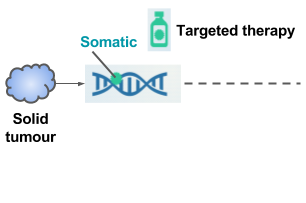
\includegraphics[scale=0.7]{somatic_precision.png}
\end{figure}
\end{frame}

\begin{frame}
\frametitle{BC Cancer Agency's OncoPanel}
\begin{figure}[t]
    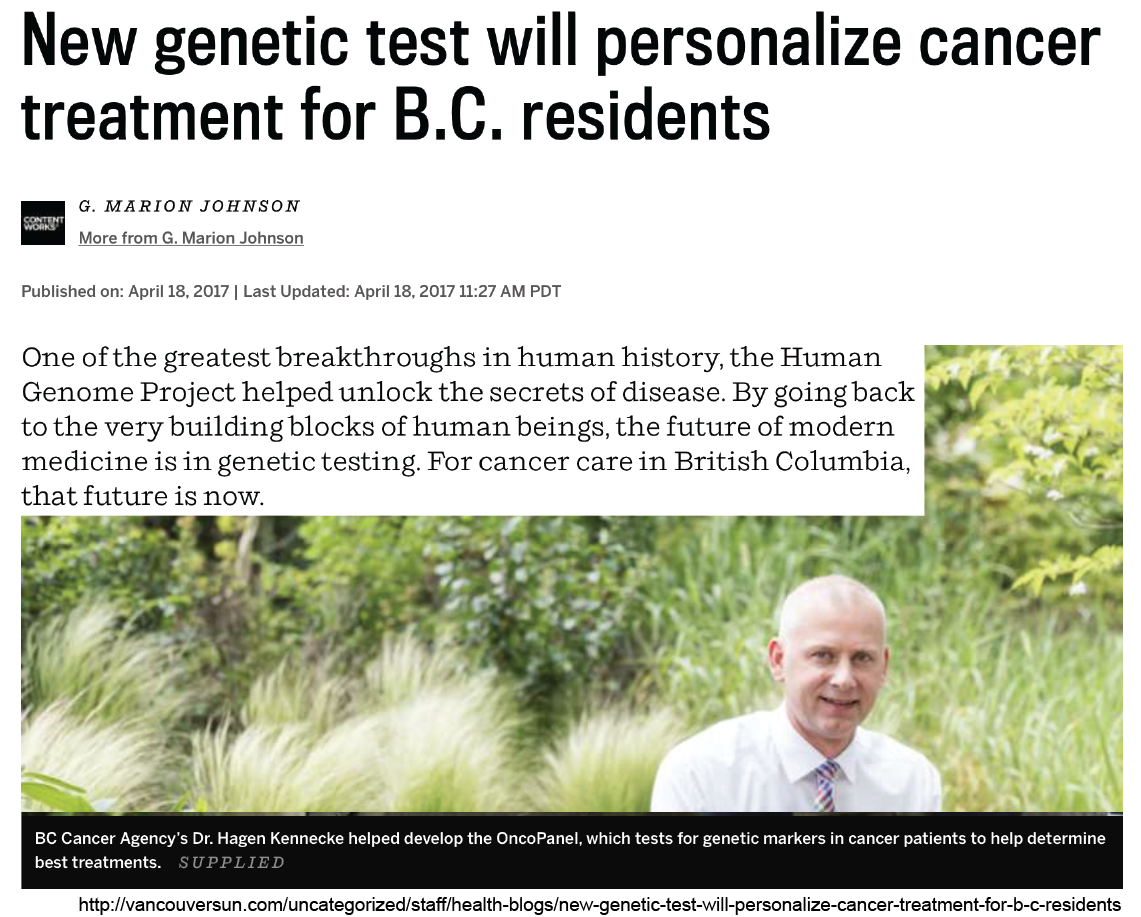
\includegraphics[scale=0.4]{oncopanel_news.png}
\end{figure}
\end{frame}

\begin{frame}
\frametitle{BC Cancer Agency's OncoPanel}
\begin{figure}[t]
    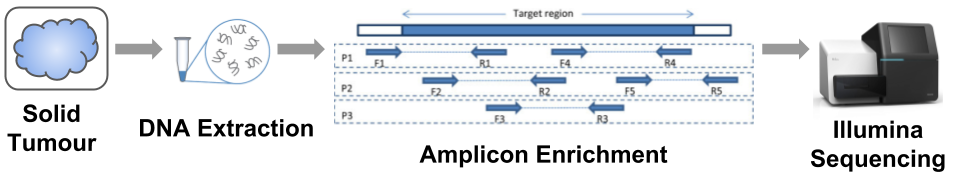
\includegraphics[scale=0.33]{oncopanel_amplicon_sequencing.png}
\end{figure}
\begin{enumerate}
\uncover<1->{\item Targeted next-generation sequencing panel for solid tumours}
\uncover<2->{\item First gene panel to be available province wide and as part of standard of care}
\end{enumerate}
\end{frame}

\begin{frame}
\frametitle{The tumour genome contains germline information}
\begin{figure}[t]
    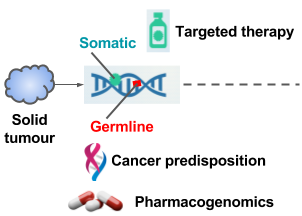
\includegraphics[scale=0.7]{germline_precision.png}
\end{figure}
\end{frame}

\begin{frame}
\frametitle{Clinical implications of germline variants}
\begin{figure}[t]
    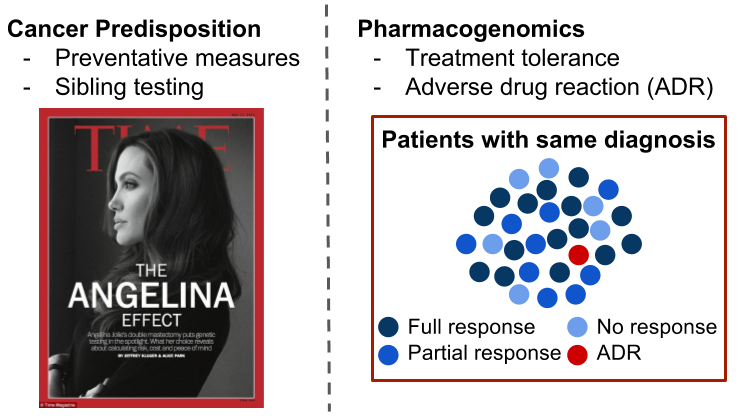
\includegraphics[scale=0.4]{precision_oncology_germline2.png}
\end{figure}
\end{frame}

\begin{frame}
\frametitle{Example: UGT1A1 promoter polymorphism leads to irinotecan toxicity}
\begin{figure}[t]
    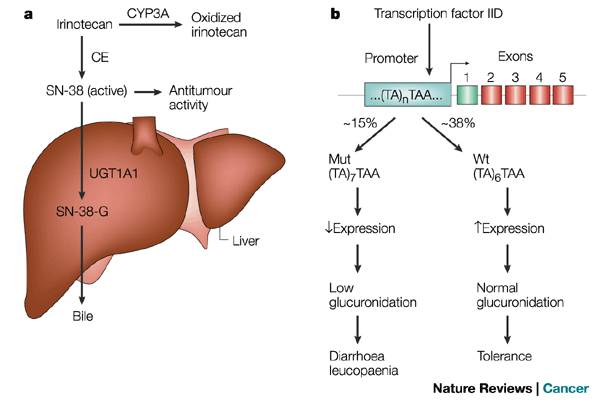
\includegraphics[scale=0.42]{ugt1a1.png}
\end{figure}
\footnotetext[1]{Relling M.V \& T. Dervieux, 2001, Nature Reviews Cancer 1, 99-108}
\end{frame}

\begin{frame}
\frametitle{Tumour-only sequencing is common in clinical laboratories}
\begin{figure}[t]
    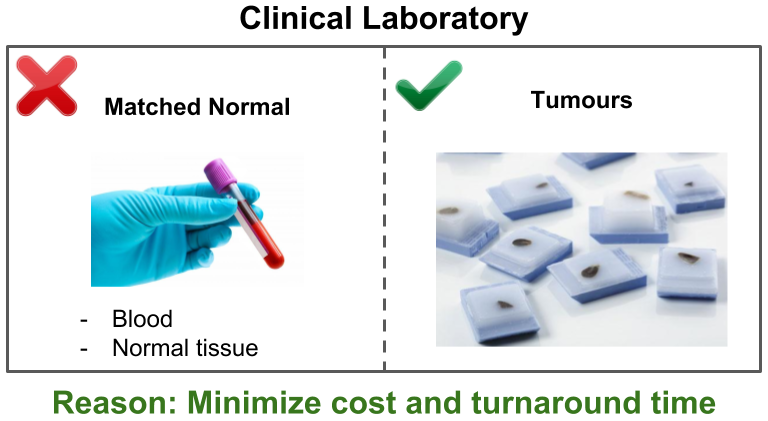
\includegraphics[scale=0.35]{clinlasb_reality.png}
\end{figure}
\end{frame}

% Research Question
\section{Research Question}
\begin{frame}
\frametitle{Research Question}
\begin{figure}[t]
    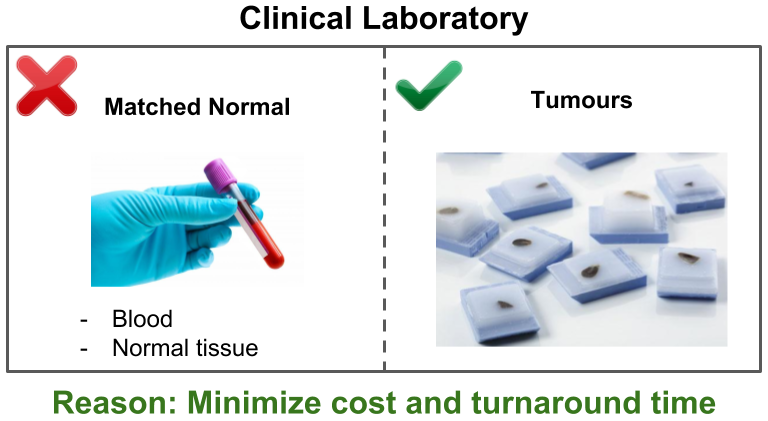
\includegraphics[scale=0.35]{clinlasb_reality.png}
\end{figure}
\centering
\uncover<2->{\textcolor{red}{Can we use tumour sequencing to screen for germline variants?}}
\end{frame}

%%%%%%%%%%%%%%%%%%%%%%%%%%%%%%%%%%%%%%%%%%%%%%%%%%%%%%%%%%%%%%%%%%%%%

\begin{frame}
\frametitle{Fix the Fixation: Technical challenges in clinical genomics}
\begin{figure}[t]
    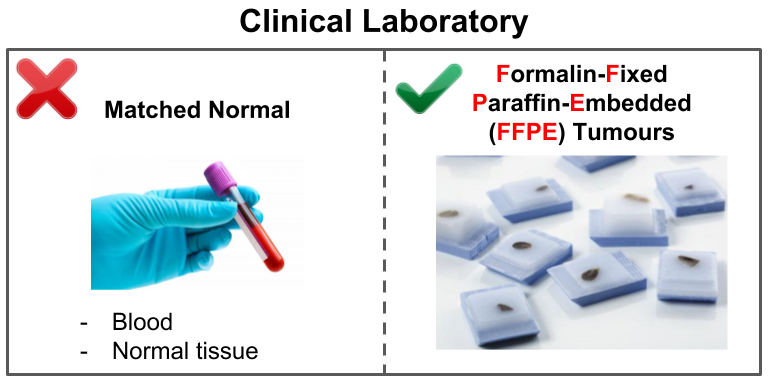
\includegraphics[scale=0.35]{clinlasb_reality_ffpe.png}
\end{figure}
\end{frame}

\begin{frame}
\frametitle{Fix the Fixation: Technical challenges in genetic testing}
\begin{figure}[t]
    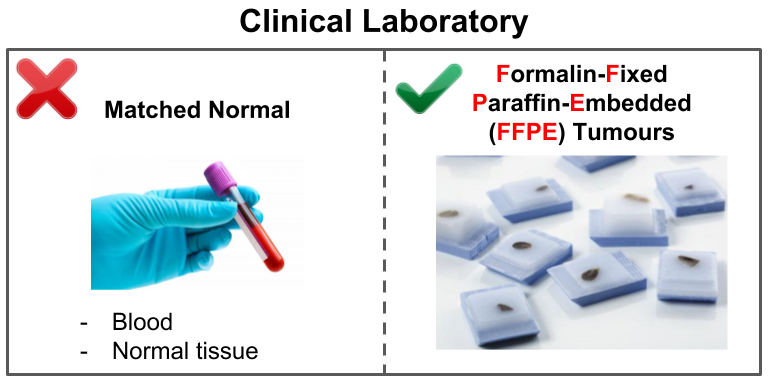
\includegraphics[scale=0.35]{clinlasb_reality_ffpe.png}
\end{figure}
Formalin-induced artifacts:
\begin{enumerate}
\uncover<1->{\item DNA fragmentation}
\uncover<2->{\item Sequence artifacts (e.g. C$>$T/G$>$A transitions)}
\end{enumerate}
\end{frame}

\begin{frame}
\frametitle{Recap}
\begin{enumerate}
\uncover<1->{\item The tumour genome contains germline information.}
\uncover<2->{\item Germline variants have clinical implications for patients and their families.}
\uncover<3->{\item Matched normal samples are rarely processed by clinical laboratories due to additional \textcolor{red}{cost} and \textcolor{red}{turnaround time.}}
\\~\\
\uncover<4->{Research question: \textcolor{red}{Can we use tumour sequencing to screen for germline variants?}}
\\~\\
\uncover<5->{\item Tumour specimens are commonly FFPE, which causes to DNA damages.}
\end{enumerate}
\end{frame}

\begin{frame}
\frametitle{Process for evaluation of genetic tests}
\begin{figure}[t]
    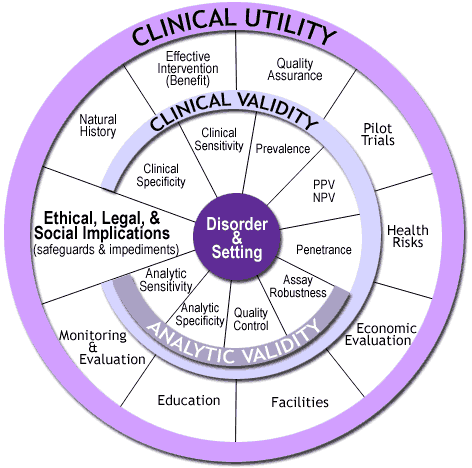
\includegraphics[scale=0.4]{ACCE_wheel.png}
\end{figure}
\end{frame}

\begin{frame}
\frametitle{Analytic Validation}
\textcolor{red}{Can we use tumour sequencing to screen for germline variants?}
\begin{figure}[t]
    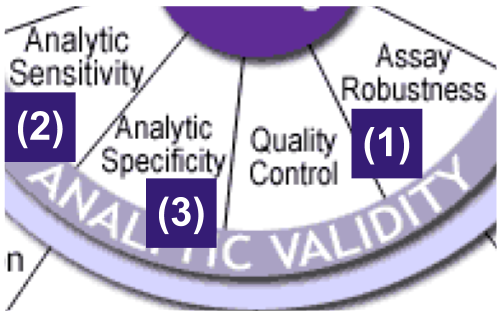
\includegraphics[scale=0.2]{wheel.png}
\end{figure}
\begin{enumerate}
\uncover<1->{\item Do sequencing results differ between FFPE specimens and blood (gold standard for germline testing)?}
\uncover<2->{\item What is the true positive rate of detecting germline variants in FFPE tumours?}
\uncover<3->{\item What is the percentage of true germline variants being referred to downstream germline testing (precision)?}
\end{enumerate}
\end{frame}

\begin{frame}
\frametitle{Study Design}
\begin{figure}[t]
    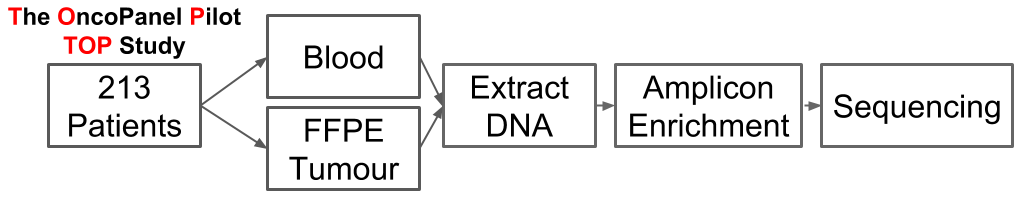
\includegraphics[scale=0.32]{study_design_general.png}
\end{figure}
\end{frame}

\begin{frame}
\frametitle{Tumour types in the TOP cohort}
\small
\begin{table}
\caption{}
\centering
      \begin{tabular}{lccc}
        \hline
        Cancer Type & Number of Cases & Percentage (\%) \\ \hline
        Colorectal & 97 & 46 \\
        Lung & 59 & 28 \\
        Melanoma & 18 & 8 \\
				Other & 17 & 8 \\
				GIST & 7 & 3 \\
				Sarcoma & 4 & 2 \\
				Neuroendocrine & 4 & 2 \\
				Cervical & 2 & 0.9 \\
				Ovarian & 2 & 0.9 \\
				Breast & 2 & 0.9 \\
				Unknown & 1 & 0.5 \\
        \hline
      \end{tabular}
\end{table}
\end{frame}

\begin{frame}
\frametitle{Cancer-related genes in the OncoPanel}
\scriptsize
\begin{table}
    \caption{}
    \centering
    \begin{tabular}{lll}
    \hline
    Gene & Protein \\
    \hline
    AKT1 & Protein kinase B \\
    ALK & Anaplastic lymphoma receptor tyrosine kinase \\
    BRAF & Serine/threonine-protein kinase B-Raf \\
    EGFR & Epidermal growth factor receptor \\
    HRAS & GTPase HRas \\
    MAPK1 & Mitogen-activated protein kinase 1 \\
    MAP2K1 & Mitogen-activated protein kinase kinase 1 \\
    MTOR & Serine/threonine-protein kinase mTOR \\
    NRAS & Neuroblastoma RAS viral oncogene homolog \\
    PDGFRA & Platelet-derived growth factor receptor alpha \\
    PIK3CA & Phosphatidylinositol-4,5-bisphosphate 3-kinase catalytic subunit alpha \\
    PTEN & Phosphatase and tensin homolog \\
    STAT1 & Signal transducer and activator of transcription 1 \\
    STAT3 & Signal transducer and activator of transcription 3 \\
    TP53 & Tumor protein P53 \\
    \hline
    \end{tabular}
\end{table}
\end{frame}

\begin{frame}
\frametitle{Pharmacogenomic genes in the OncoPanel}
\scriptsize
\begin{table}
    \caption{}
    \centering
    \begin{tabular}{llll}
    \hline
    Gene & Protein & Chemotherapy \\
    \hline
    DPYD & Dihydropyrimidine dehydrogenase & 5-FU \\
    GSTP1 & Glutathione S-rransferase pi 1 & Oxaliplatin \\
    MTHFR & Methylenetetrahydrofolate reductase & 5-FU \\
    TYMP & Thymidine phosphorylase & 5-FU \\
    TYMS & Thymidylate synthetase & 5-FU \\
    UGT1A1 & Uridine diphosphate (UDP)-glucuronosyl transferase 1A1 & Irinotecan \\
    \hline
    \end{tabular}
\end{table}
\end{frame}

%%%%%%%%%%%%%%%%%%%%%%%%%%%%%%%%%%%%%%%%%%%%%%%%%%%%%%%%%%%%%%%%%%%%%
%%%%%%%%%%%%%%%%%%%%%%%%%%%%%%%%%%%%%%%%%%%%%%%%%%%%%%%%%%%%%%%%%%%%%
% Project aims
\section{Project Aims}

\begin{frame}
\frametitle{Project Aims}
\textcolor{red}{Can we use tumour sequencing to screen for germline variants?}
\begin{enumerate}
\uncover<1->{\item \textcolor{red}{Assay QC:} Compare efficiency in amplicon enrichment and sequencing results between blood and FFPE specimens}
\uncover<2->{\item \textcolor{red}{Sensitivity:} Determine the true positive rate for detection of germline variants in FFPE tumours}
\uncover<3->{\item \textcolor{red}{Precision:} Determine the percentage of true germline variants referred for downstream germline testing}
\end{enumerate}
\end{frame}

%%%%%%%%%%%%%%%%%%%%%%%%%%%%%%%%%%%%%%%%%%%%%%%%%%%%%%%%%%%%%%%%%%%%%
% Project Aim 1
\section{Aim 1}
\begin{frame}
\frametitle{Aim 1: Compare efficiency in amplicon enrichment and sequencing results between blood and FFPE specimens}
\begin{figure}[t]
    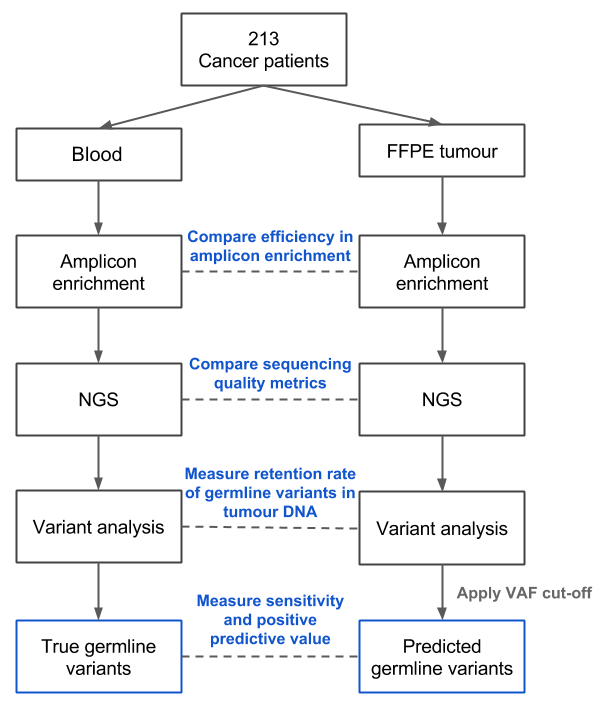
\includegraphics[scale=0.32]{study_design.png}
\end{figure}
\end{frame}

%%%%%%%%%%%%%%%%%%%%%%%%%%%%%%%%%%%%%%%%%%%%%%%%%%%%%%%%%%%%%%%%%%%%%
\begin{frame}
\frametitle{Formalin fixation causes DNA fragmentation}
\begin{figure}[t]
    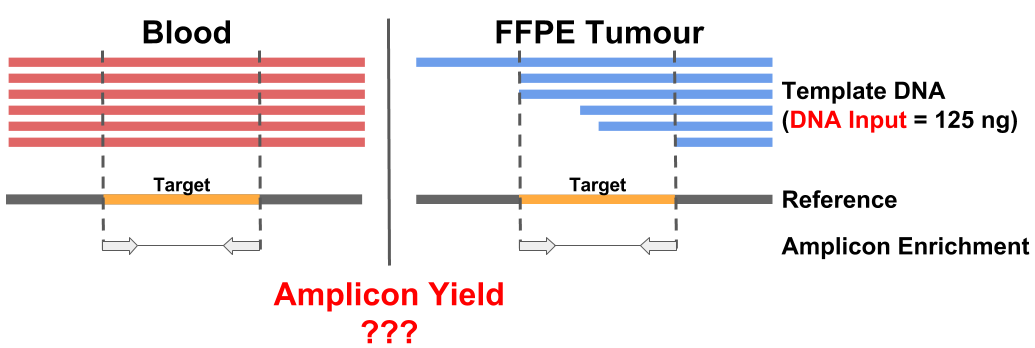
\includegraphics[scale=0.32]{fragmentation.png}
\end{figure}
\end{frame}

%%%%%%%%%%%%%%%%%%%%%%%%%%%%%%%%%%%%%%%%%%%%%%%%%%%%%%%%%%%%%%%%%%%%%
\begin{frame}
\frametitle{Correlation between DNA input and amplicon yield}
\begin{figure}[t]
    \begin{columns}
    \column{7cm}
    \centering
    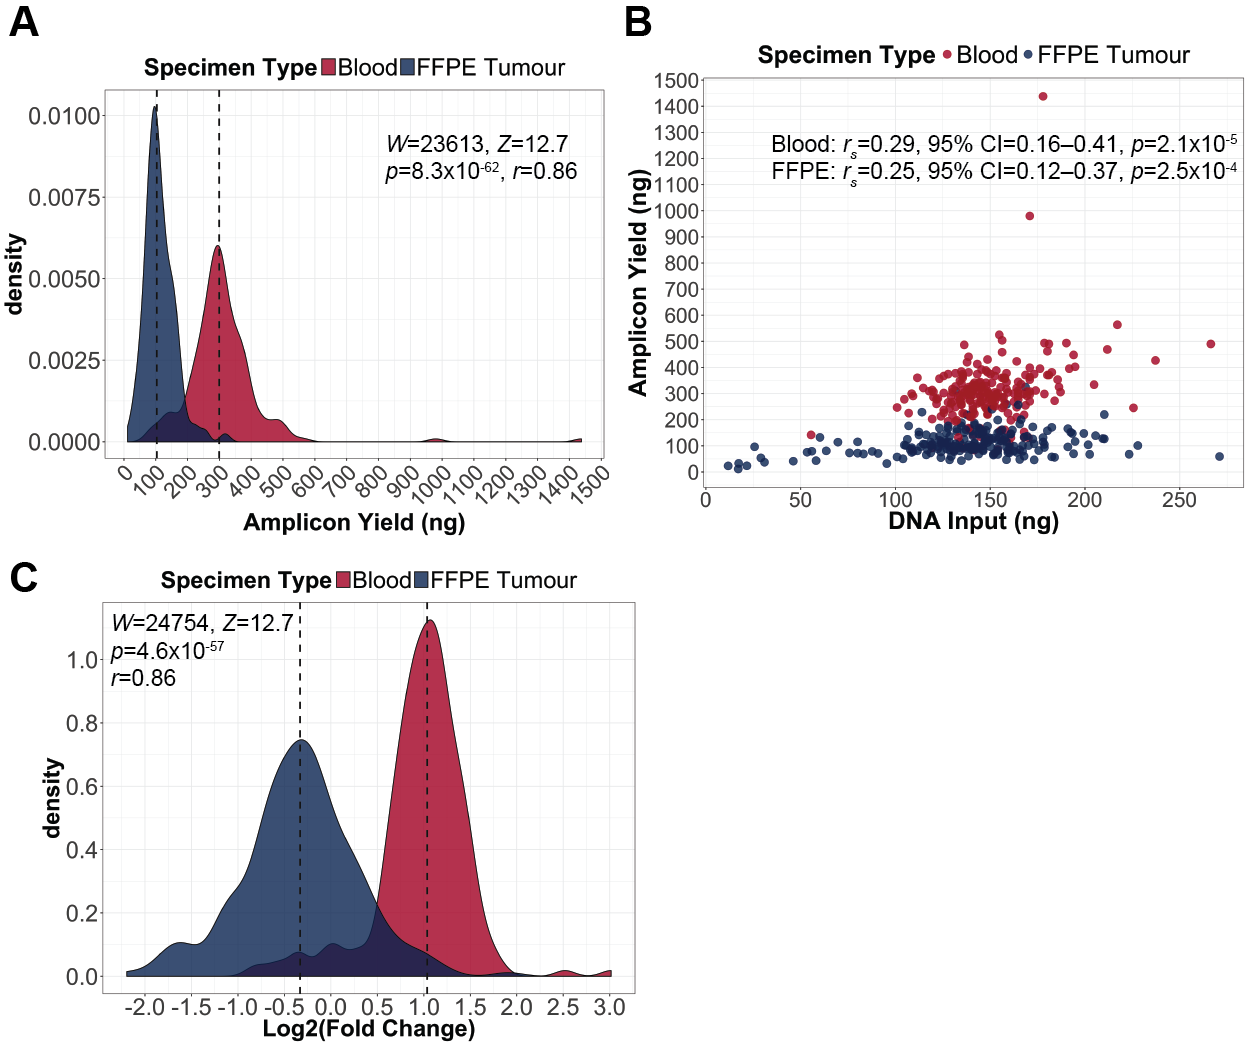
\includegraphics[scale=0.7]{dna_input_amp_yield.png}%
    \column{5cm}
    \centering
    Enrichment efficiency:
    \[
    log2\frac{\text{Amplicon Yield}}{\text{DNA Input}}
    \]
    \end{columns}
\end{figure}
\end{frame}

%%%%%%%%%%%%%%%%%%%%%%%%%%%%%%%%%%%%%%%%%%%%%%%%%%%%%%%%%%%%%%%%%%%%%
\begin{frame}
\frametitle{Reduced efficiency in amplicon enrichment is observed in FFPE specimens}
\begin{figure}[t]
    \begin{columns}
    \column{7cm}
    \centering
    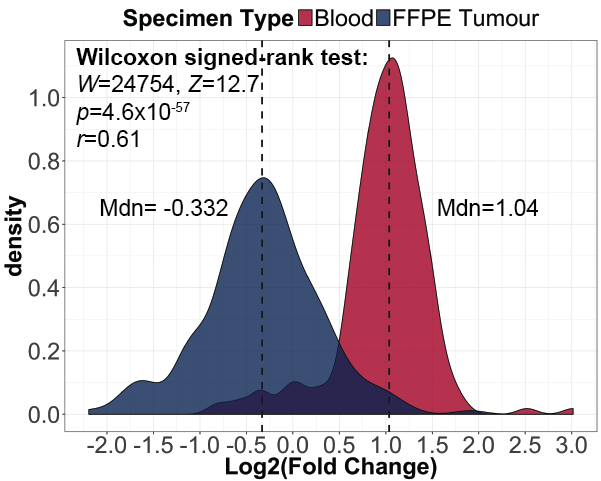
\includegraphics[scale=0.7]{dna_input_amp_yield_fc.png}%
    \column{5cm}
    \centering
    Enrichment efficiency:
    \[
    log2\frac{\text{Amplicon Yield}}{\text{DNA Input}}
    \]
    \end{columns}
\end{figure}
\end{frame}

%%%%%%%%%%%%%%%%%%%%%%%%%%%%%%%%%%%%%%%%%%%%%%%%%%%%%%%%%%%%%%%%%%%%%
\begin{frame}
\frametitle{Read Alignments}
\begin{figure}[t]
    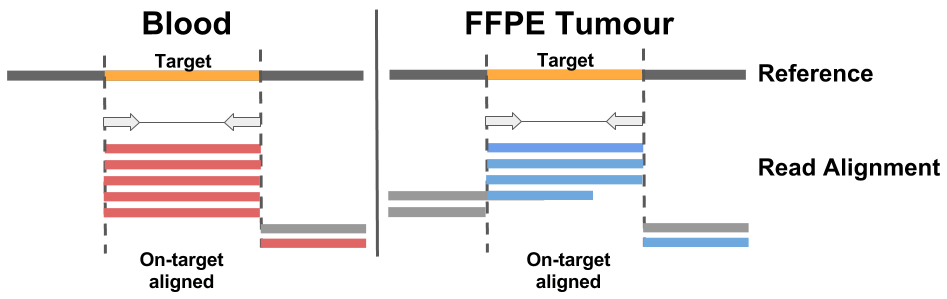
\includegraphics[scale=0.35]{ontarget_aligned.png}
\end{figure}
\end{frame}

%%%%%%%%%%%%%%%%%%%%%%%%%%%%%%%%%%%%%%%%%%%%%%%%%%%%%%%%%%%%%%%%%%%%%
\begin{frame}
\frametitle{Percentage of on-target aligned reads is comparable between specimen types}
\begin{figure}[t]
    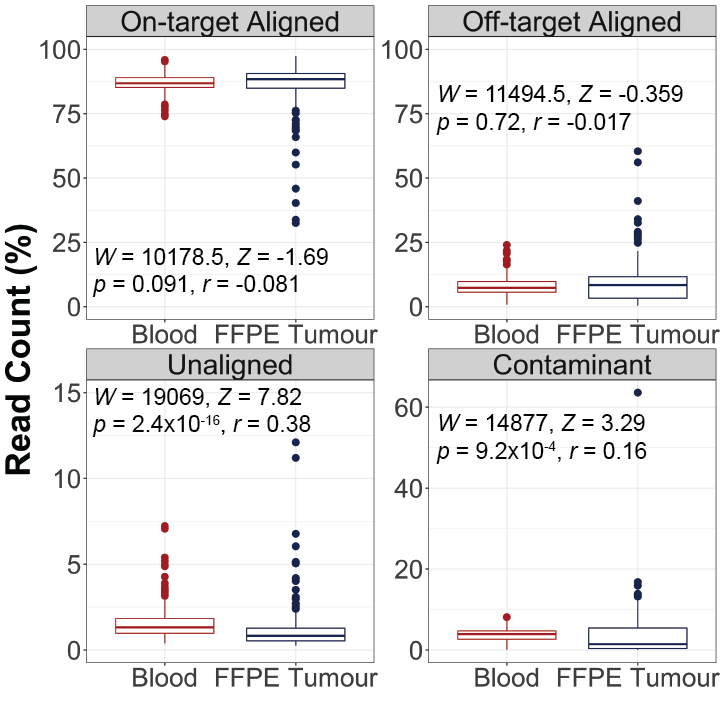
\includegraphics[scale=0.55]{alignment_pct.png}
\end{figure}
\end{frame}

%%%%%%%%%%%%%%%%%%%%%%%%%%%%%%%%%%%%%%%%%%%%%%%%%%%%%%%%%%%%%%%%%%%%%
\begin{frame}
\frametitle{Per base coverage statistics}
\begin{figure}[t]
    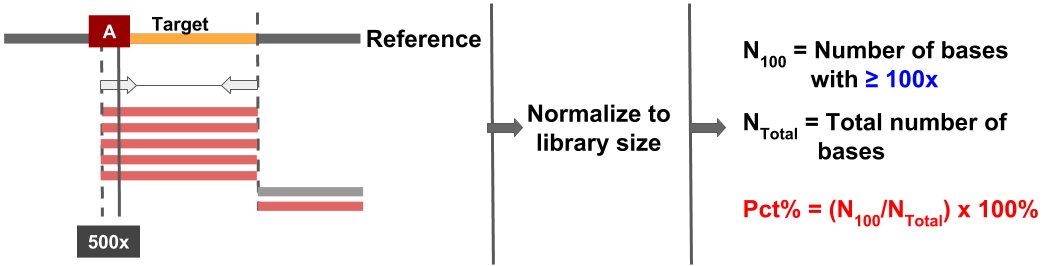
\includegraphics[scale=0.3]{per_base.png}
\end{figure}
\end{frame}

%%%%%%%%%%%%%%%%%%%%%%%%%%%%%%%%%%%%%%%%%%%%%%%%%%%%%%%%%%%%%%%%%%%%%
\begin{frame}
\frametitle{Percentage of target bases is significantly different at all coverage thresholds}
\begin{figure}[t]
    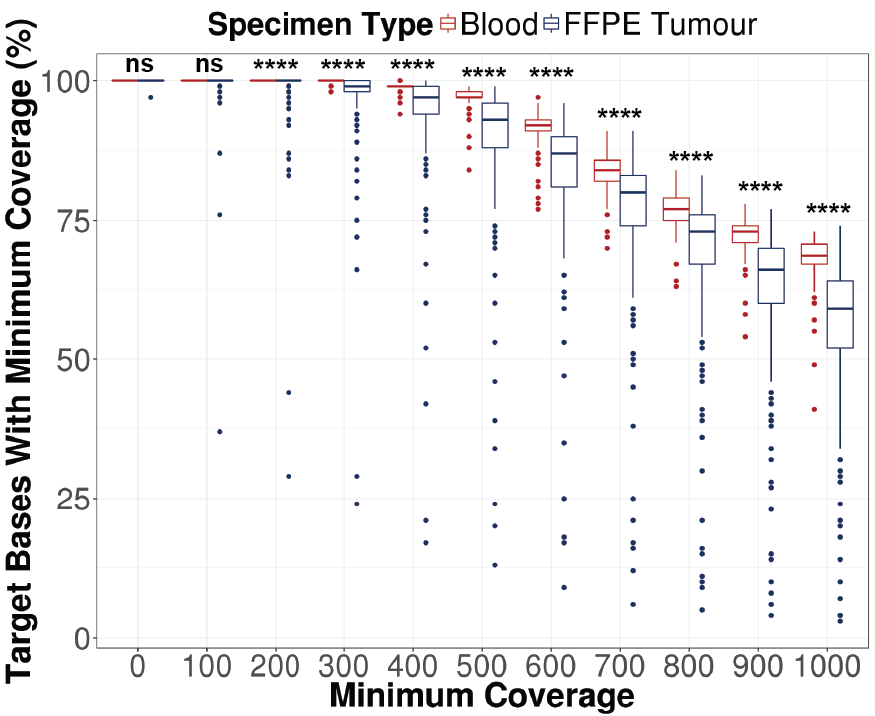
\includegraphics[scale=0.48]{coverage_stats.png}
    \caption{\scriptsize Wilcoxon signed-rank test, ****\textit{p} $<$ 0.0001, ***\textit{p} $<$ 0.001, **\textit{p} $<$ 0.01, *\textit{p} $<$ 0.05, ns = not significant}
\end{figure}
\end{frame}

%%%%%%%%%%%%%%%%%%%%%%%%%%%%%%%%%%%%%%%%%%%%%%%%%%%%%%%%%%%%%%%%%%%%%
\begin{frame}
\frametitle{OncoPanel consists of 416 amplicons}
\begin{figure}[t]
    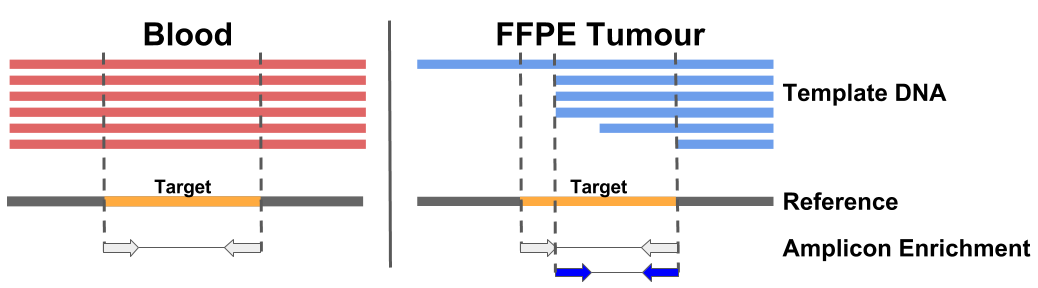
\includegraphics[scale=0.3]{amplicon_fragmentation.png}
\end{figure}
Shorter amplicons might yield greater coverage depth in FFPE specimens due to fragmentation damages in template DNA.
\end{frame}

%%%%%%%%%%%%%%%%%%%%%%%%%%%%%%%%%%%%%%%%%%%%%%%%%%%%%%%%%%%%%%%%%%%%%
\begin{frame}
\frametitle{Analysis of Amplicon Coverage Depth}
\begin{figure}[t]
    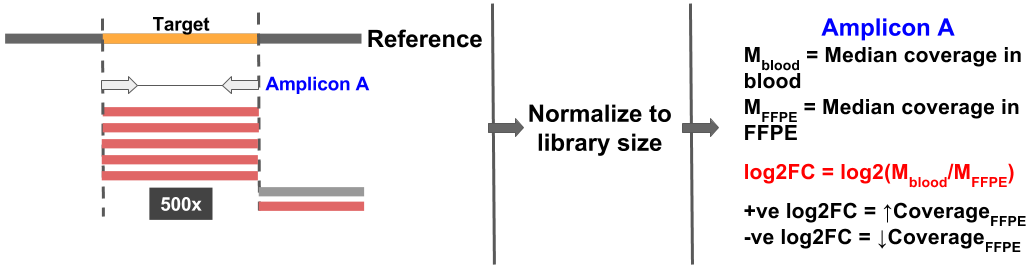
\includegraphics[scale=0.3]{amplicon_coverage.png}
\end{figure}
Comparison of amplicon coverage was performed with the Wilcoxon signed-rank test.
\end{frame}

%%%%%%%%%%%%%%%%%%%%%%%%%%%%%%%%%%%%%%%%%%%%%%%%%%%%%%%%%%%%%%%%%%%%%
\begin{frame}
\frametitle{There are more amplicons with lower coverage depth in FFPE specimens relative to blood specimens}
\begin{figure}[t]
    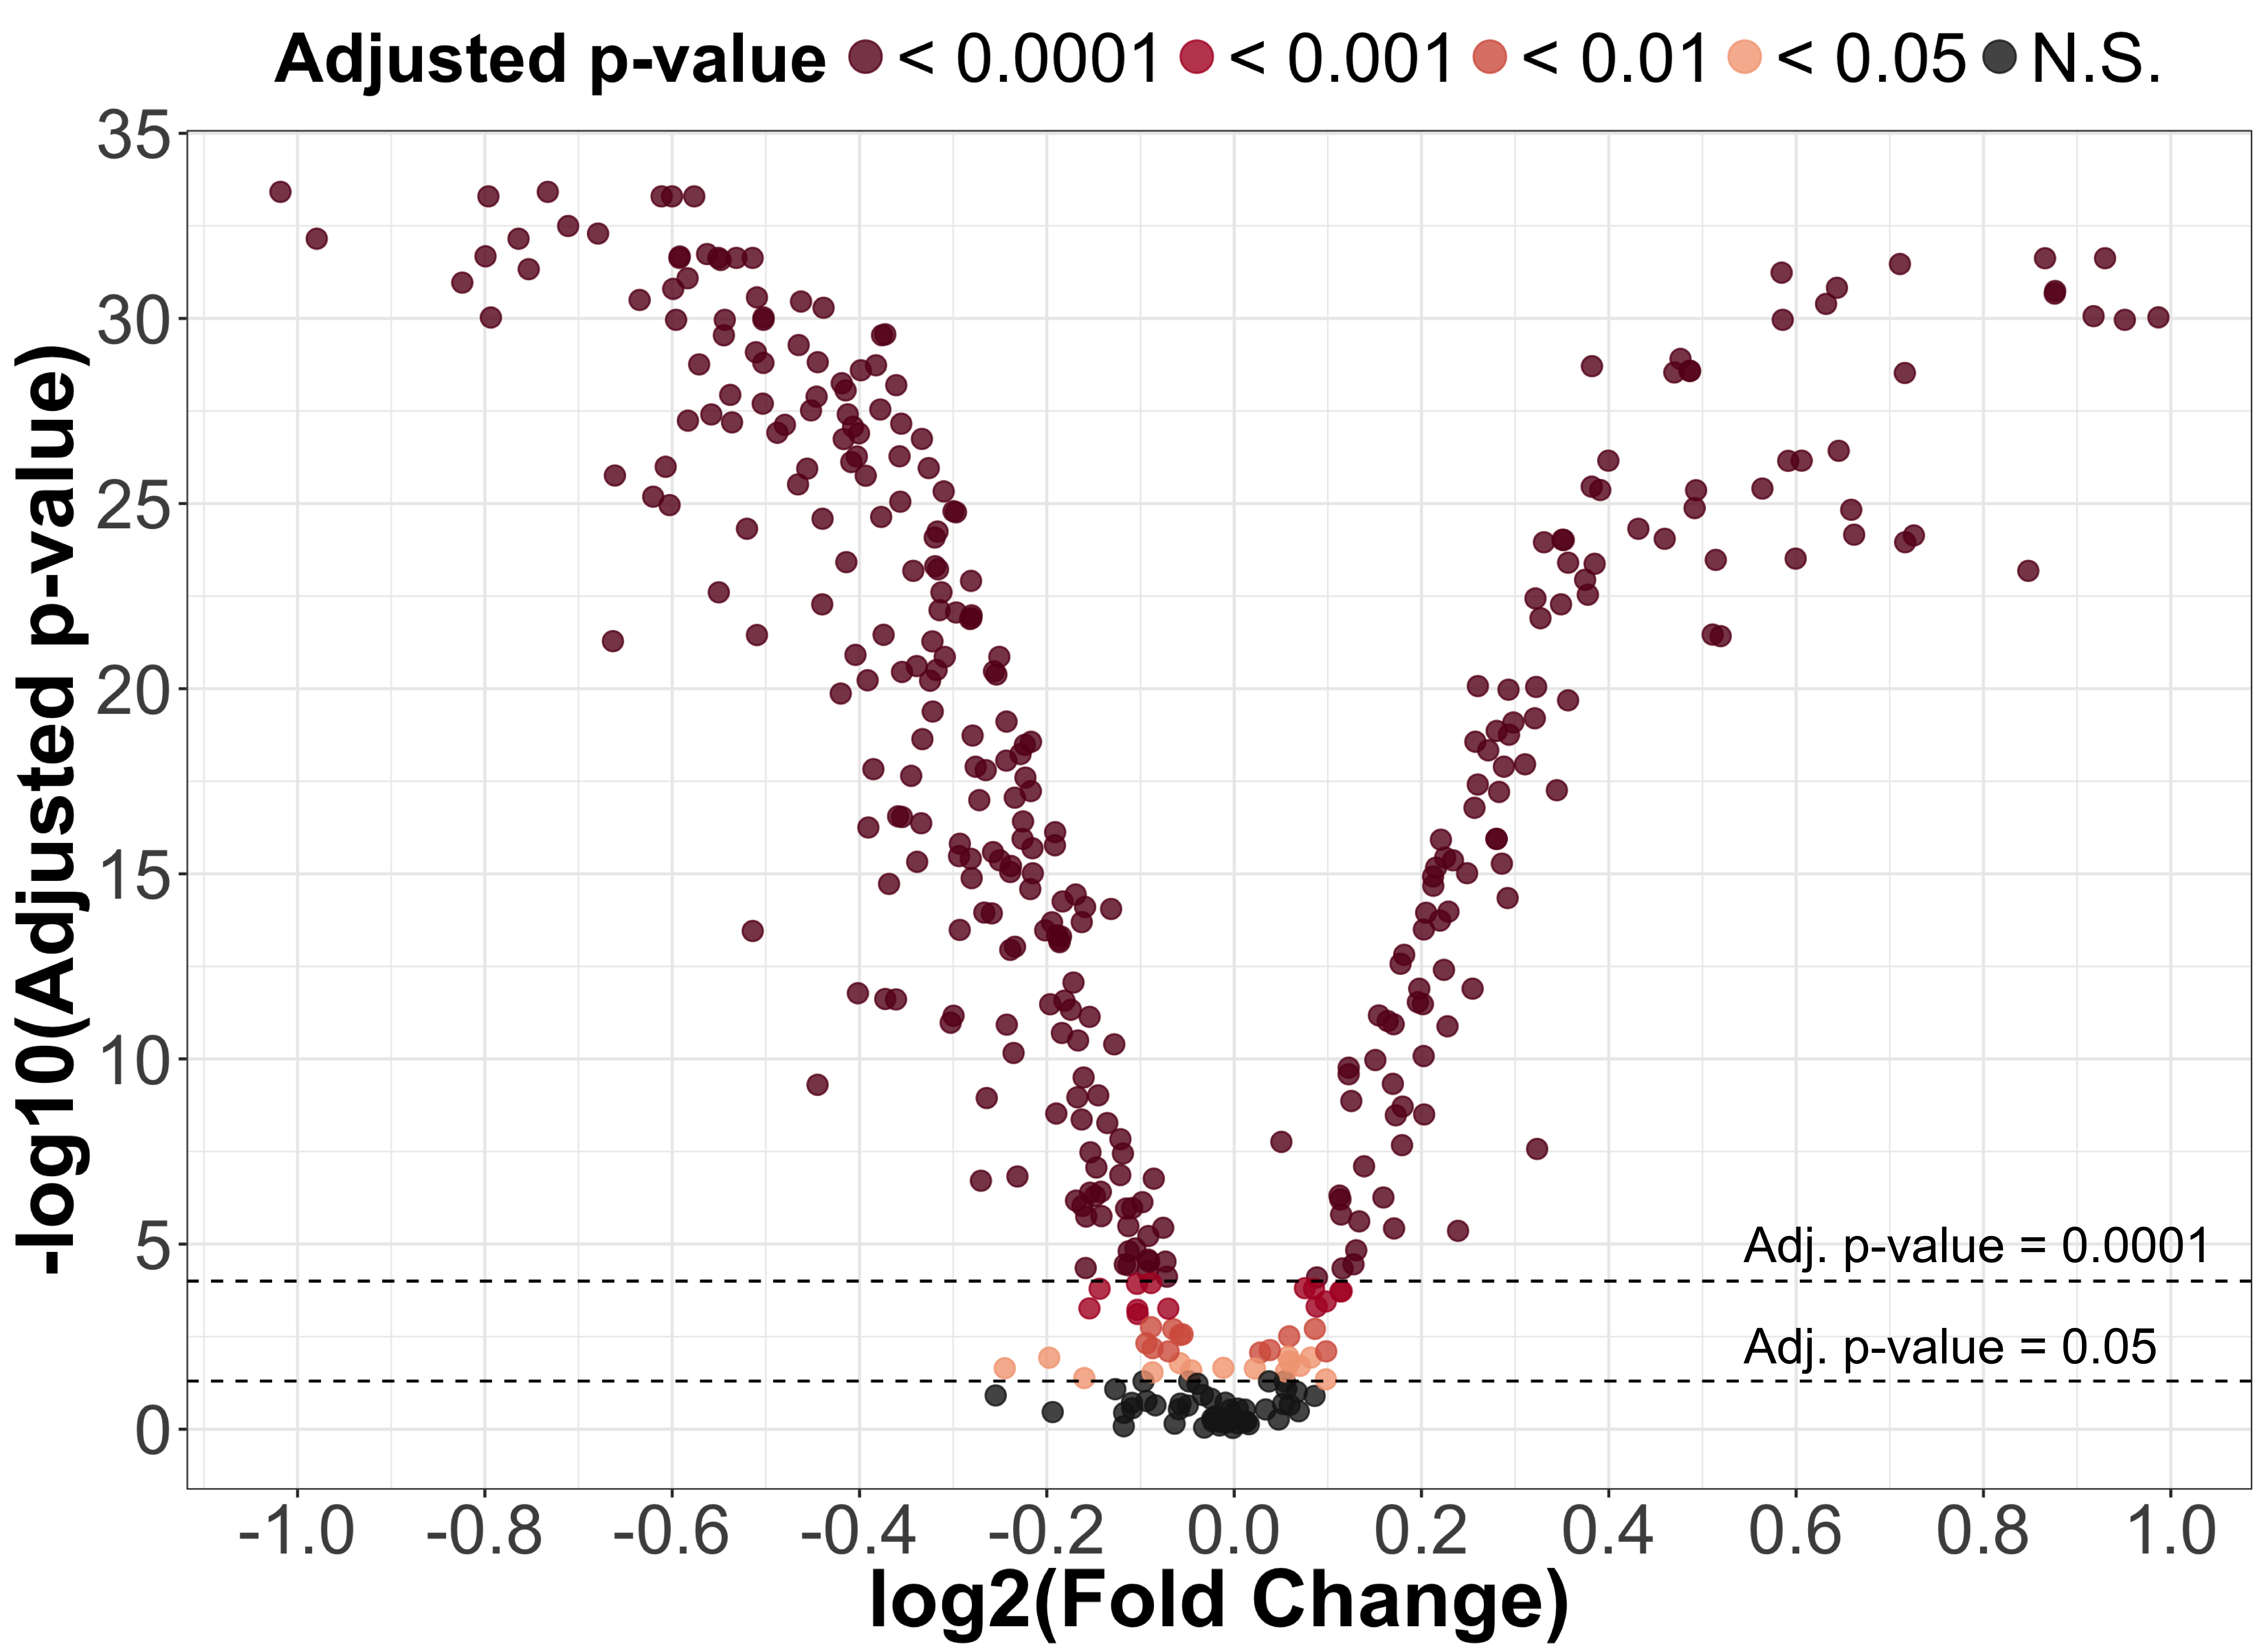
\includegraphics[scale=0.065]{amp_norm_depth_med_wilcoxon_volcano.png}
    \caption{\scriptsize Adj. \textit{p}-value = Wilcoxon signed-rank test with Benjamini Hochberg correction}
\end{figure}
\end{frame}

%%%%%%%%%%%%%%%%%%%%%%%%%%%%%%%%%%%%%%%%%%%%%%%%%%%%%%%%%%%%%%%%%%%%%
\begin{frame}
\frametitle{Decreased amplicon coverage in FFPE specimens is correlated with increased amplicon length}
\begin{figure}[t]
    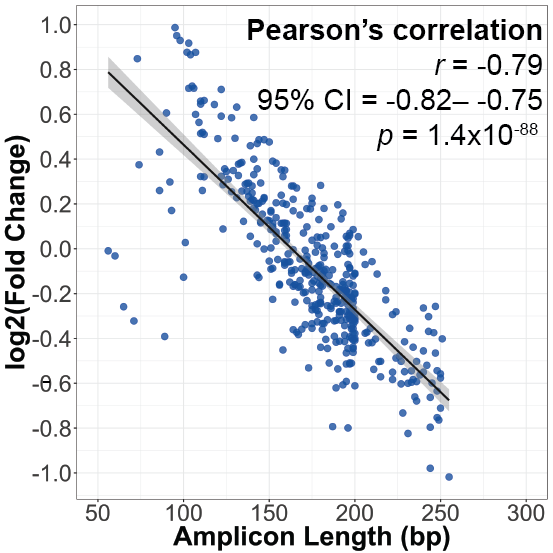
\includegraphics[scale=0.7]{amp_cov_lm_len_fc.png}
\end{figure}
\end{frame}

%%%%%%%%%%%%%%%%%%%%%%%%%%%%%%%%%%%%%%%%%%%%%%%%%%%%%%%%%%%%%%%%%%%%%
\begin{frame}
\frametitle{Decreased amplicon coverage in FFPE specimens is correlated with increased amplicon GC content}
\begin{figure}[t]
    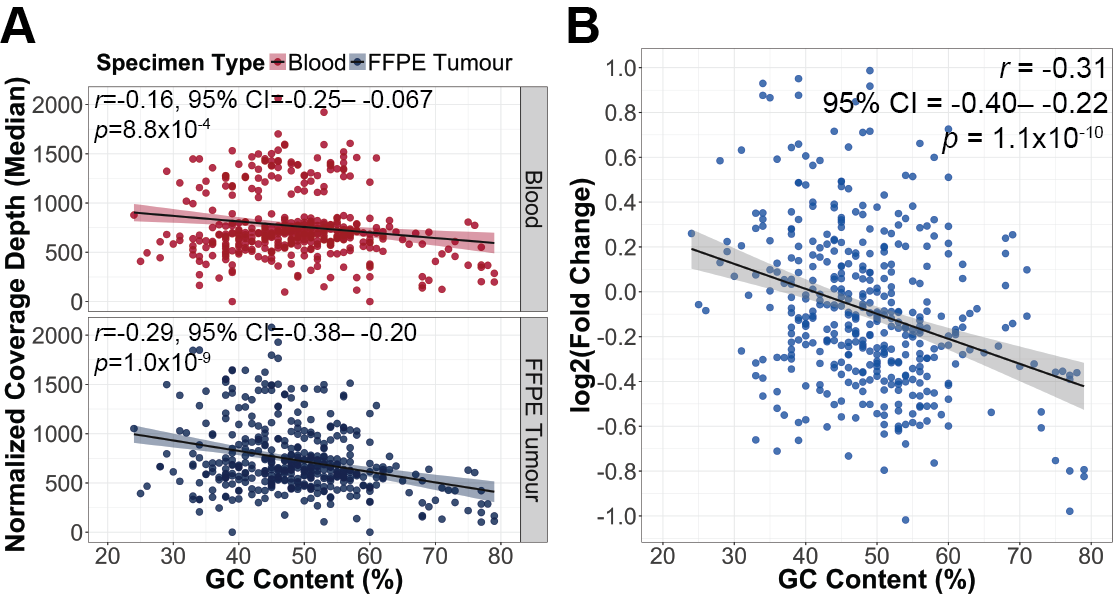
\includegraphics[scale=0.7]{amp_cov_lm_gc.png}
\end{figure}
\end{frame}

%%%%%%%%%%%%%%%%%%%%%%%%%%%%%%%%%%%%%%%%%%%%%%%%%%%%%%%%%%%%%%%%%%%%%
\begin{frame}
\frametitle{Reduced amplicon coverage in FFPE specimens is more pronounced for longer amplicons}
\scriptsize
\begin{table}
\caption{Multiple regression of amplicon length and GC content as predictors for log2FC between amplicon coverage in FFPE specimens and blood.}
\label{multiple_regression}
\centering
      \begin{tabular}{l|ccccl}
        Variable & Unstandardized & S.E. & Standardized & \textit{p}-value
        \\
        \hline
        Length (bp) & \num{-7.24e-3} & \num{2.54e-4} & \num{-7.75e-1} & \num{2.47e-99}
				\\
				GC Content (\%) & \num{-9.92e-3} & \num{9.77e-4} & \num{-2.77e-1} & \num{8.70e-22}
				\\
				\hline
				\\
				 & \multicolumn{4}{r}{Intercept = 1.66, Adjusted R\textsuperscript{2} = 0.695}
				\\
				 & \multicolumn{4}{r}{\textit{F}(2, 411) = 471, \textit{p}-value = \num{4.65e-107}}
				\\
				\hline
      \end{tabular} \\
\end{table}
A change in 1 standard deviation of amplicon length has $>$2x the impact on log2FC than a 1 standard deviation change in amplicon GC content.
\end{frame}

%%%%%%%%%%%%%%%%%%%%%%%%%%%%%%%%%%%%%%%%%%%%%%%%%%%%%%%%%%%%%%%%%%%%%
\begin{frame}
\frametitle{Formalin fixation induces deamination of cytosine bases}
\begin{figure}[t]
    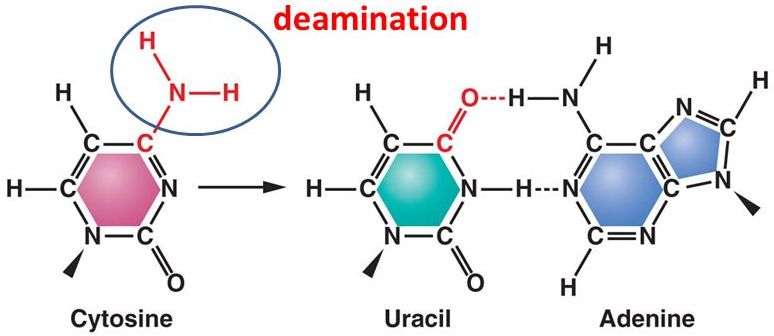
\includegraphics[scale=0.4]{deamination_explanation.jpg}
\end{figure}
\footnotetext[1]{Klug and Cummings, 1997}
\end{frame}

%%%%%%%%%%%%%%%%%%%%%%%%%%%%%%%%%%%%%%%%%%%%%%%%%%%%%%%%%%%%%%%%%%%%%
\begin{frame}
\frametitle{Deamination effects lead to increased C$>$T/G$>$A transitions in FFPE specimens (Wilcoxon signed-rank test)}
\begin{figure}[t]
    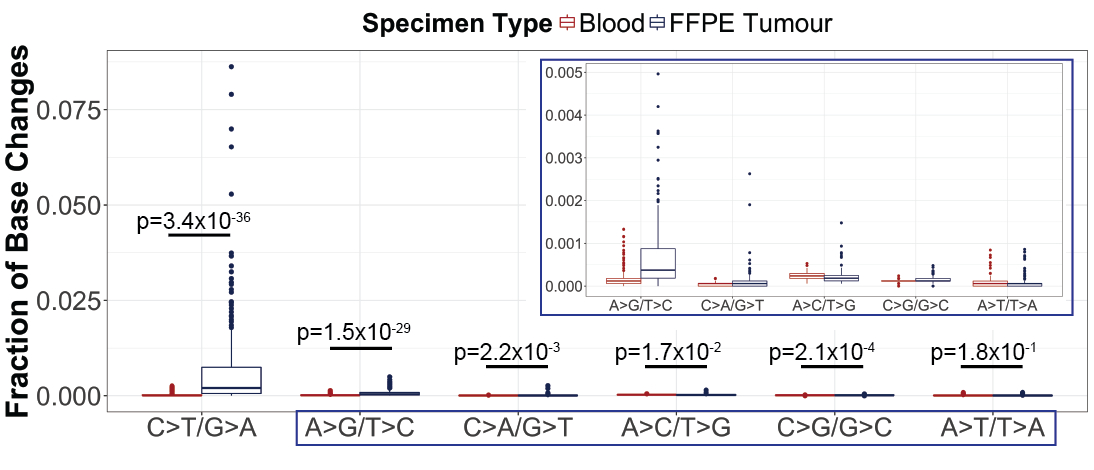
\includegraphics[scale=0.58]{deamination_effect.png}
\end{figure}
\end{frame}

%%%%%%%%%%%%%%%%%%%%%%%%%%%%%%%%%%%%%%%%%%%%%%%%%%%%%%%%%%%%%%%%%%%%%
\begin{frame}
\frametitle{Deamination effects lead to increased C$>$T/G$>$A transitions in FFPE specimens (Wilcoxon signed-rank test, fold change)}
\begin{figure}[t]
    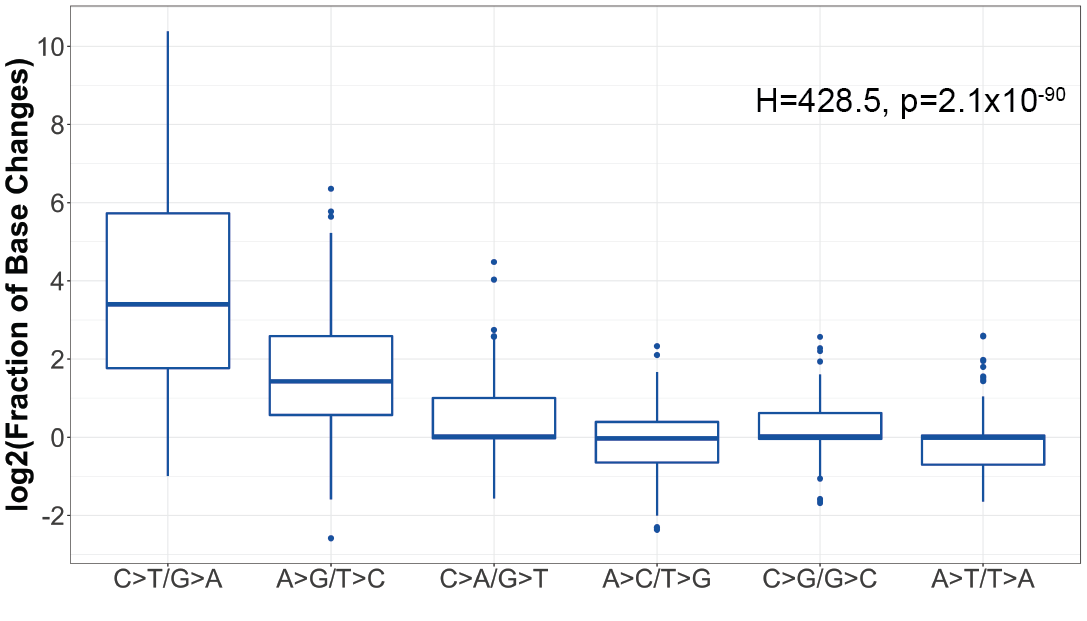
\includegraphics[scale=0.58]{deamination_effect_blood_fc.png}
\end{figure}
\end{frame}

%%%%%%%%%%%%%%%%%%%%%%%%%%%%%%%%%%%%%%%%%%%%%%%%%%%%%%%%%%%%%%%%%%%%%
\begin{frame}
\frametitle{Deamination effects lead to increased C$>$T/G$>$A transitions in FFPE specimens at low allele frequency (Wilcoxon signed-rank test)}
\begin{figure}[t]
    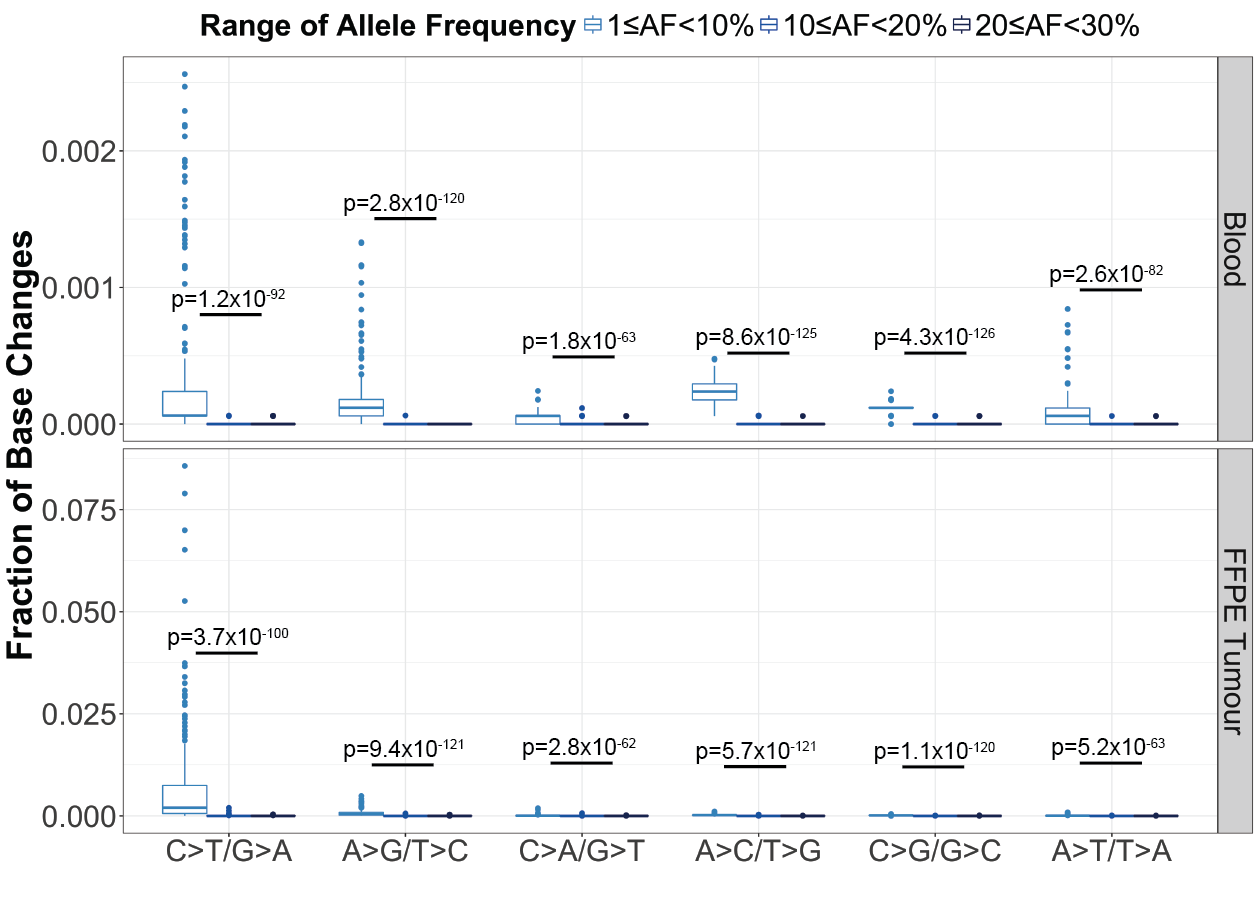
\includegraphics[scale=0.4]{deamination_effect_af_range.png}
\end{figure}
\end{frame}

%%%%%%%%%%%%%%%%%%%%%%%%%%%%%%%%%%%%%%%%%%%%%%%%%%%%%%%%%%%%%%%%%%%%%
\begin{frame}
\frametitle{Deamination effects lead to increased C$>$T/G$>$A transitions in FFPE specimens at low allele frequency (Wilcoxon signed-rank test, enlarged figure)}
\begin{figure}[t]
    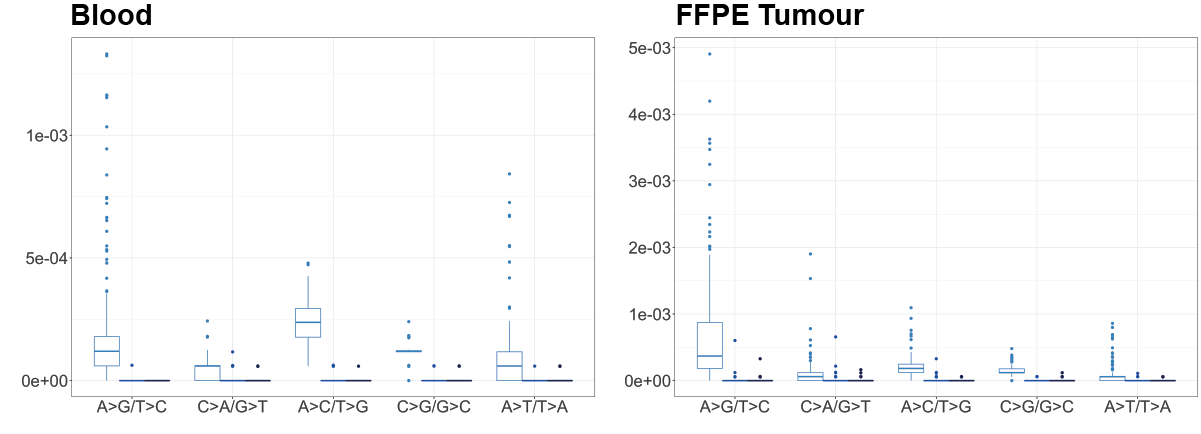
\includegraphics[scale=0.52]{deamination_effect_af_range_big.png}
\end{figure}
\end{frame}

%%%%%%%%%%%%%%%%%%%%%%%%%%%%%%%%%%%%%%%%%%%%%%%%%%%%%%%%%%%%%%%%%%%%%
\begin{frame}
\frametitle{Increased age of paraffin block results in reduced amplicon yield}
\begin{figure}[t]
    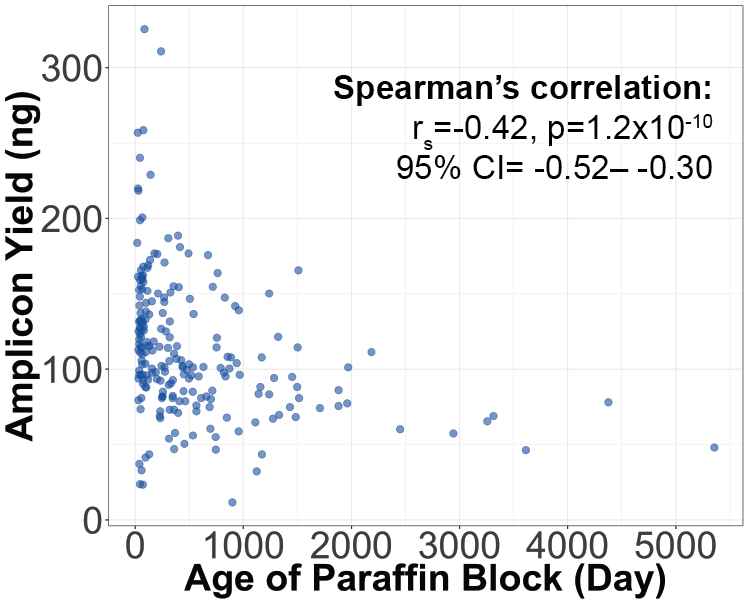
\includegraphics[scale=0.55]{deamination_effect_age_amp.png}
\end{figure}
\end{frame}

%%%%%%%%%%%%%%%%%%%%%%%%%%%%%%%%%%%%%%%%%%%%%%%%%%%%%%%%%%%%%%%%%%%%%
\begin{frame}
\frametitle{Increased age of paraffin block results in elevated events of C$>$T/G$>$A sequence artifacts (Spearman's correlation)}
\begin{figure}[t]
    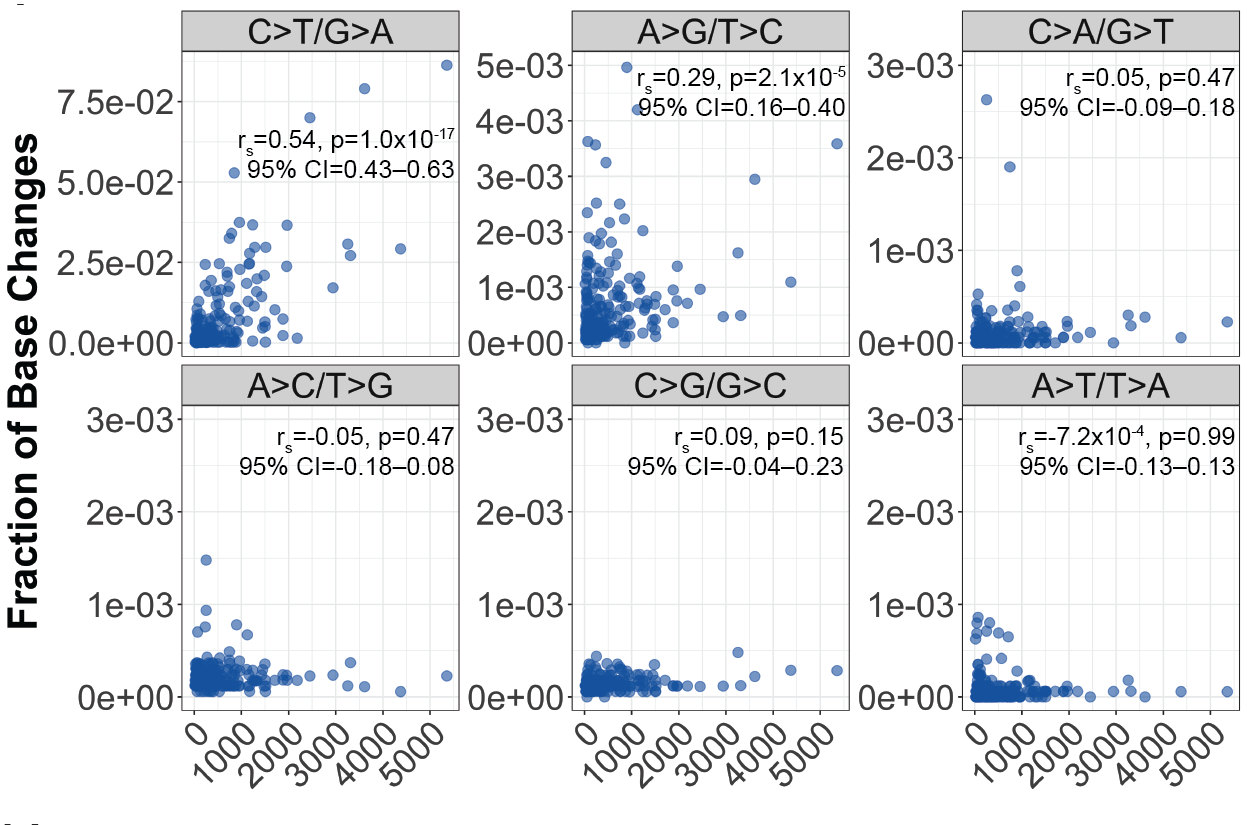
\includegraphics[scale=0.45]{deamination_effect_age_artifact.png}
\end{figure}
\end{frame}

%%%%%%%%%%%%%%%%%%%%%%%%%%%%%%%%%%%%%%%%%%%%%%%%%%%%%%%%%%%%%%%%%%%%%
\begin{frame}
\begin{table}
\caption{Determination of correlation between pre-sequencing variables and sequencing results using Spearman's correlation. Top values represent Spearman's \textit{rho} and 95\% confidence interval in brackets, whereas bottom values represent \textit{p}-value. Asterisk(*) indicates significance level of \textit{p}-value $<$ 0.05.}
\tiny
\centering
      \begin{tabular}{l|l|l|l|ll}
        Variable & Amplicon & Age of Paraffin & Fraction of & Average Per Base
        \\
				 & Yield (ng) & Block (Day) & C$>$T/G$>$A & Normalized Coverage
				\\
        \hline
        Age of Paraffin & -0.42 (-0.52-- -0.30) & & &
				\\
				Block (Day) & \num{5.2e-7}\mbox{*} & & &
        \\
				\hline
				Fraction of & -0.72 (-0.77-- -0.65) & 0.54 (0.61--0.75) & &
				\\
				C$>$T/G$>$A & \num{1.9e-11}\mbox{*} & \num{6.3e-35}\mbox{*} & &
				\\
				\hline
				Average Per Base & 0.69 (0.61--0.75) & -0.47 (-0.57-- -0.36) & -0.80 (-0.84-- -0.75) &
				\\
				Normalized Coverage & \num{8.5e-20}\mbox{*} & \num{4.7e-7}\mbox{*} & \num{7.5e-17}\mbox{*} &
				\\
				\hline
				On-target & 0.58 (0.48--0.66) & -0.35 (-0.46-- -0.23) & -0.57 (-0.65-- -0.47) & 0.73 (0.66--0.79)
				\\
				Aligned Reads (\%) & \num{2.1e-13}\mbox{*} & \num{8.2e-3}\mbox{*} & \num{4.2e-8}\mbox{*} & \num{3.1e-58}\mbox{*}
				\\
				\hline
      \end{tabular} \\
\end{table}
\end{frame}

%%%%%%%%%%%%%%%%%%%%%%%%%%%%%%%%%%%%%%%%%%%%%%%%%%%%%%%%%%%%%%%%%%%%%
\begin{frame}
\frametitle{Summary for Aim 1}
\begin{enumerate}
\uncover<1->{\item Efficiency in amplicon enrichment is lower in FFPE compared to blood.}
\uncover<2->{\item Percentage of on-target aligned reads (\%) is comparable between blood and FFPE specimens.}
\uncover<3->{\item There is discrepancy in coverage depth between blood and FFPE specimens.}
\uncover<4->{\item Shorter amplicons achieve greater coverage in FFPE specimens compared to longer amplicons.}
\uncover<5->{\item Increased C$>$T/G$>$A transitions are observed in FFPE specimens, and this increase is correlated with increased age of paraffin blocks.}
\end{enumerate}
\end{frame}

%%%%%%%%%%%%%%%%%%%%%%%%%%%%%%%%%%%%%%%%%%%%%%%%%%%%%%%%%%%%%%%%%%%%%
%%%%%%%%%%%%%%%%%%%%%%%%%%%%%%%%%%%%%%%%%%%%%%%%%%%%%%%%%%%%%%%%%%%%%
% Project Aim 2
\section{Aim 2}
\begin{frame}
\frametitle{Aim 2: Determine the true positive rate for detection of germline variants in FFPE tumours (sensitivity)}
\begin{figure}[t]
    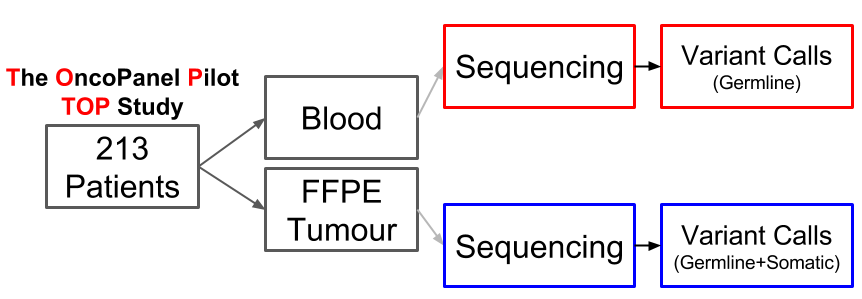
\includegraphics[scale=0.3]{study_design_sens.png}
\end{figure}
\end{frame}

\begin{frame}
\frametitle{Variant calling pipeline}
\begin{figure}[t]
    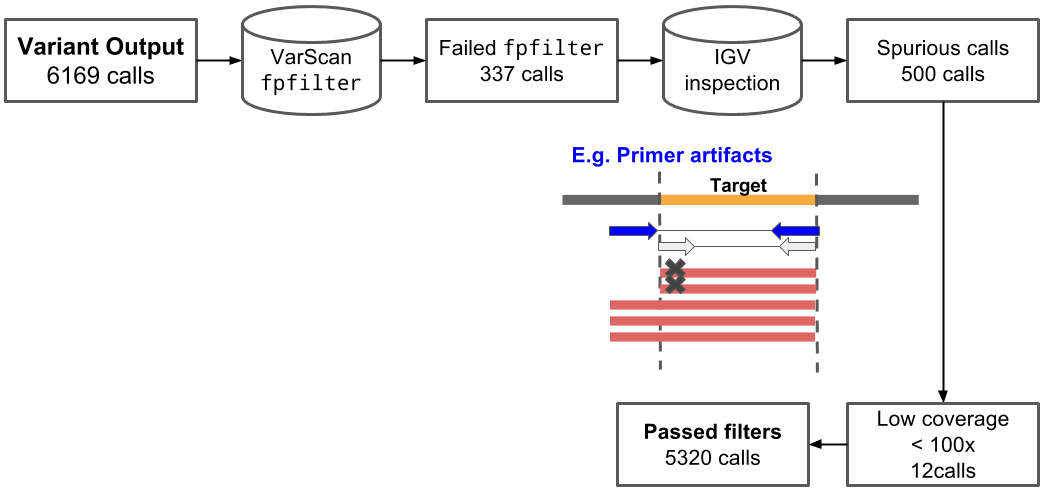
\includegraphics[scale=0.3]{variant_pipeline.png}
\end{figure}
\end{frame}

\begin{frame}
\frametitle{Germline variants are highly concordant between blood and FFPE specimens}
\begin{figure}[t]
    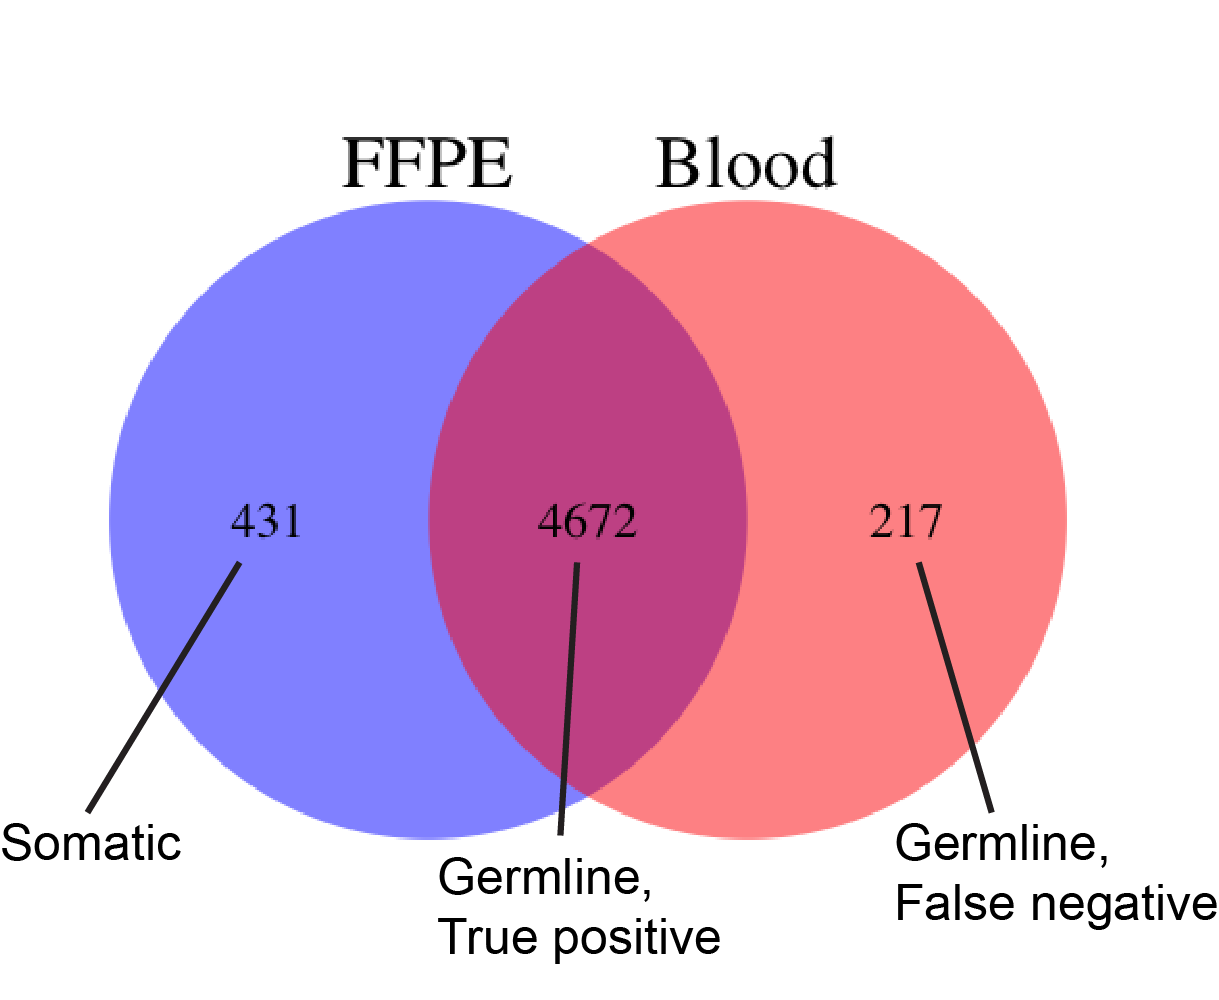
\includegraphics[scale=0.32]{variant_conc_venn.png}
\end{figure}
\centering
True positive rate = 4672/(217+4672) = 0.956
\end{frame}

%%%%%%%%%%%%%%%%%%%%%%%%%%%%%%%%%%%%%%%%%%%%%%%%%%%%%%%%%%%%%%%%%%%%%
% Project Aim 3
\section{Aim 3}
\begin{frame}
\frametitle{Aim 3: Determine the percentage of true germline variants referred for downstream germline testing (precision/positive predictive value)}
\begin{figure}[t]
    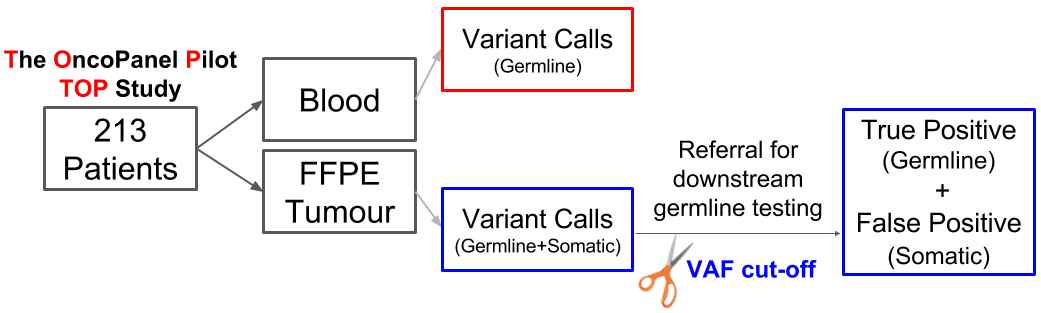
\includegraphics[scale=0.3]{study_design_ppv.png}
\end{figure}
\end{frame}

\begin{frame}
\frametitle{VAF of germline and somatic variants in FFPE tumour}
\begin{figure}[t]
    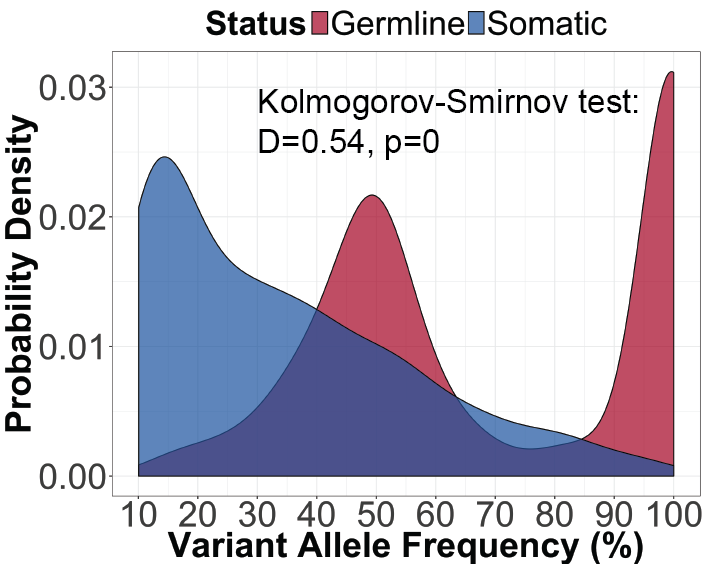
\includegraphics[scale=0.6]{germline_somatic_ppv.png}
\end{figure}
\end{frame}

\begin{frame}
\frametitle{VAF of germline variants in blood and FFPE tumour}
\begin{figure}[t]
    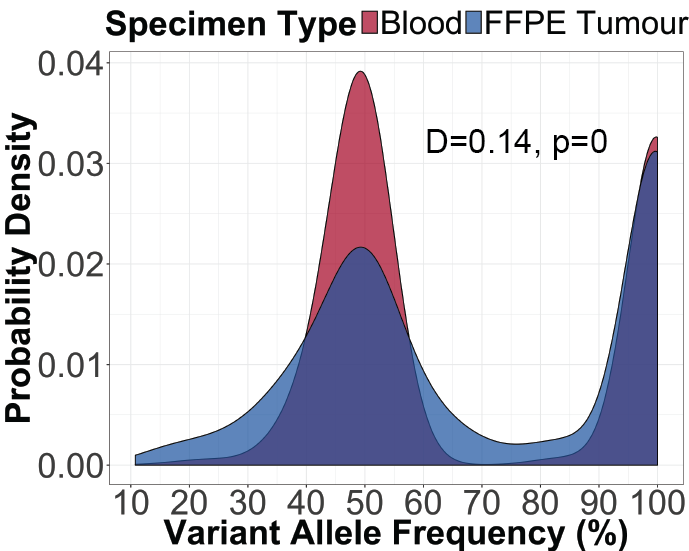
\includegraphics[scale=0.6]{germline_vaf_sens.png}
\end{figure}
\end{frame}

\begin{frame}
\frametitle{Reduced sensitivity in detection of germline variants at 40\% VAF}
\begin{table}
\centering
\tiny
\begin{tabular}{cllcclllccl}
        \hline
				\multicolumn{1}{l}{ }
				&
				\multicolumn{4}{l}{Blood}
				&&
				\multicolumn{4}{l}{FFPE Tumour}
        \\
				\cline{2-5}\cline{7-10}
        VAF (\%) & FN\mbox{*} & TP\mbox{**} & Sensitivity & 95\% CI && FN\mbox{*} & TP\mbox{**} & Sensitivity & 95\% CI
        \\
        \hline
        10 & 0 & 2461 & 1.0 & 1.0--1.0 && 0 & 2428 & 1.0 & 1.0--1.0
        \\
        15 & 2 & 2459 & 1.0 & 1.0-1.0 && 12 & 2416 & 1.0 & 0.99--1.0
        \\
        20 & 3 & 2458 & 1.0 & 1.0--1.0 && 48 & 2380 & 0.98 & 0.97--0.99
        \\
        25 & 15 & 2446 & 0.99 & 0.99--1.00 && 79 & 2349 & 0.97 & 0.96--0.97
        \\
        30 & 20 & 2441 & 0.99 & 0.99--1.00 && 121 & 2307 & 0.95 & 0.94--0.96
        \\
        35 & 33 & 2428 & 0.99 & 0.98--0.99 && 197 & 2231 & 0.92 & 0.91--0.93
        \\
        40 & 107 & 2354 & 0.96 & 0.95--0.96 && 328 & 2100 & 0.86 & 0.85--0.88
        \\
        45 & 234 & 2227 & 0.90 & 0.89--0.92 && 470 & 1958 & 0.81 & 0.79--0.82
        \\
				\hline
      \end{tabular} \\
      *FN = False negative; **TP = True positive
\end{table}
\end{frame}

\begin{frame}
\frametitle{Reduced sensitivity in detection of germline variants at 40\% VAF}
\begin{figure}[t]
    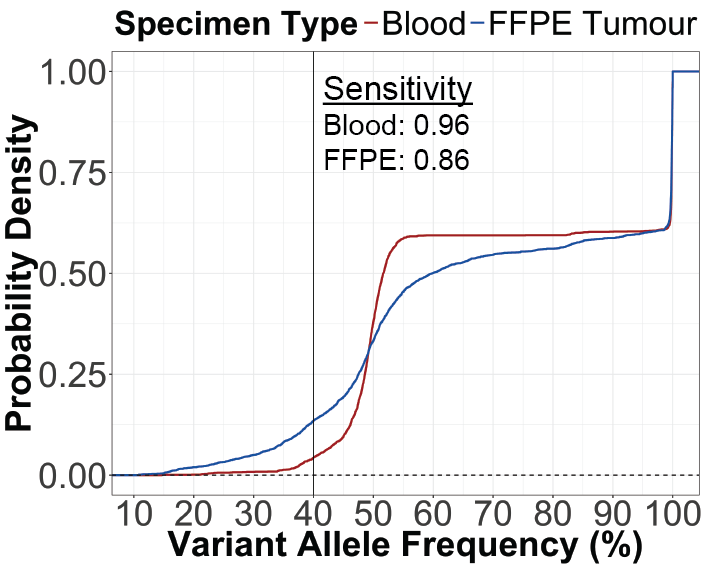
\includegraphics[scale=0.6]{germline_vaf_sens_cdf.png}
\end{figure}
\end{frame}

\begin{frame}
\frametitle{High positive predictive value can be achieved for referral of germline variants to downstream confirmatory testing}
\centering
\scriptsize
\begin{table}
\centering
      \begin{tabular}{ccccccl}
        \hline
        VAF (\%) & FP* & TP** & Total Calls & Positive Predictive Value & 95\% CI
        \\
        \hline
        10 & 431 & 2428 & 2859 & 0.85 & 0.84--0.86
        \\
        15 & 319 & 2416 & 2735 & 0.88 & 0.87--0.90
        \\
        20 & 273 & 2380 & 2653 & 0.90 & 0.88--0.91
        \\
        25 & 245 & 2349 & 2594 & 0.91 & 0.89--0.92
        \\
        30 & 203 & 2307 & 2510 & 0.92 & 0.91--0.93
        \\
        35 & 178 & 2231 & 2409 & 0.93 & 0.91--0.94
        \\
        40 & 146 & 2100 & 2246 & 0.93 & 0.92--0.94
        \\
        45 & 118 & 1958 & 2076 & 0.94 & 0.93--0.95
        \\
				\hline
      \end{tabular}
      *FP = False positive; **TP = True positive
\end{table}
\end{frame}

\begin{frame}
\frametitle{High positive predictive value can be achieved for referral of germline variants to downstream confirmatory testing}
\begin{figure}[t]
    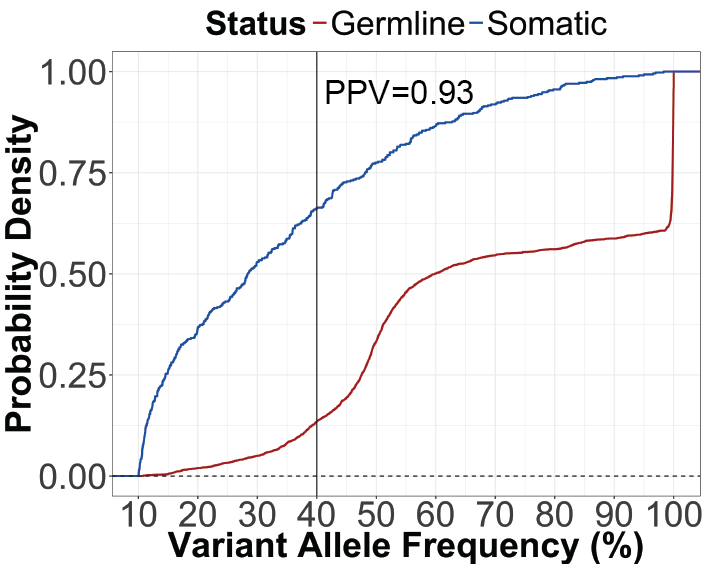
\includegraphics[scale=0.6]{germline_somatic_ppv_cdf.png}
\end{figure}
\end{frame}

%%%%%%%%%%%%%%%%%%%%%%%%%%%%%%%%%%%%%%%%%%%%%%%%%%%%%%%%%%%%%%%%%%%%%
% Conclusion
\section{Conclusions}
\begin{frame}
\frametitle{Conclusions}
\begin{enumerate}
\uncover<1->{\item Formalin-induced DNA damages are detectable in NGS data.}
\uncover<2->{\item Germline variants are highly concordant between blood and FFPE specimens (\textcolor{red}{TPR = 0.956}).}
\uncover<3->{\item At 40\% VAF threshold, sensitivity for detection of germline variants in FFPE tumour is \textcolor{red}{0.86} and the positive predictive value for referral to downstream confirmatory testing is \textcolor{red}{0.93}.}
\end{enumerate}
\end{frame}

%%%%%%%%%%%%%%%%%%%%%%%%%%%%%%%%%%%%%%%%%%%%%%%%%%%%%%%%%%%%%%%%%%%%%
\begin{frame}
\frametitle{Acknowledgements}
Karsan lab past and current members
\\~\\

Committee:
\begin{itemize}
  \item Dr. Ryan Morin
  \item Dr. Martin Hirst
\end{itemize}

Centre of Clinical Genomics:
\begin{itemize}
  \item Liz Starks
  \item Jillian Slind
  \item Hadrien Jouet
\end{itemize}
\end{frame}

\begin{frame}
\frametitle{Acknowledgements}
GSC sequencing team
\\~\\
Cancer Genetics Lab
\\~\\
Patients
\end{frame}

\begin{frame}
\frametitle{Acknowledgements}
\begin{figure}[t]
    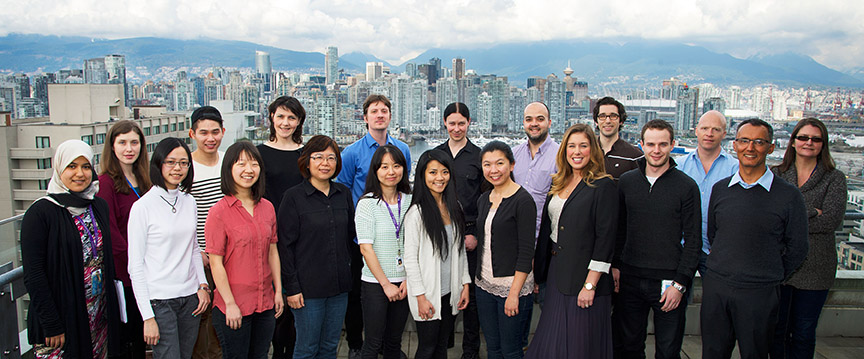
\includegraphics[scale=0.3]{Karsan-Lab_4470_web}
\end{figure}
\end{frame}

% Supplementary
%%%%%%%%%%%%%%%%%%%%%%%%%%%%%%%%%%%%%%%%%%%%%%%%%%%%%%%%%%%%%%%%%%%%%
\begin{frame}
\frametitle{Percentage of target bases is significantly different at all coverage thresholds}
\begin{table}
\centering
\tiny
      \begin{tabular}{llllllll}
        \hline
				\multicolumn{1}{l}{ }
				&
				\multicolumn{2}{l}{Blood}
				&&
				\multicolumn{2}{l}{FFPE Tumour}
				&
				\multicolumn{2}{l}{ } \\
				\cline{2-3}\cline{5-6}
        Threshold & Median (\%) & Range (\%) && Median (\%) & Range (\%) & \textit{p} ($<$ 0.05\textsuperscript{*}) & \textit{r}
				\\
				\hline
				$\geq$ 0x & 100.0 & 100.0--100.0 && 100.0 & 97.0--100.0 & 1.0 & 0.068
				\\
				$\geq$ 100x & 100.0 & 100.0--100.0 && 100.0 & 37.0--100.0 & \num{2.3e-4}\textsuperscript{*} & 0.25
				\\
				$\geq$ 200x & 100.0 & 100.0--100.0 && 100.0 & 29.0--100.0 & \num{2.9e-11}\textsuperscript{*} & 0.41
				\\
				$\geq$ 300x & 100.0 & 98.0--100.0 && 99.0 & 24.0--100.0 & \num{4.1e-18}\textsuperscript{*} & 0.55
				\\
				$\geq$ 400x & 99.0 & 94.0--100.0 && 97.0 & 17.0--100.0 & \num{5.0e-28}\textsuperscript{*} & 0.68
				\\
				$\geq$ 500x & 97.0 & 84.0--99.0 && 89.5 & 13.0--99.0 & \num{2.1e-38}\textsuperscript{*} & 0.77
				\\
				$\geq$ 600x & 92.0 & 77.0--97.0 && 87.0 & 9.0--96.0 & \num{1.5e-32}\textsuperscript{*} & 0.72
				\\
				$\geq$ 700x & 84.0 & 70.0--91.0 && 80.0 & 6.0--91.0 & \num{5.7e-25}\textsuperscript{*} & 0.65
				\\
				$\geq$ 800x & 77.0 & 63.0-84.0 && 73.0 & 5.0--83.0 &  \num{4.7e-27}\textsuperscript{*} & 0.67
				\\
				$\geq$ 900x & 73.0 & 54.0--78.0 && 66.0 & 4.0--77.0 &  \num{4.6e-40}\textsuperscript{*} & 0.78
				\\
				$\geq$ 1000x & 68.5 & 41.0--73.0 && 59.0 & 3.0-74.0 & \num{3.6e-42}\textsuperscript{*} & 0.79
				\\
				\hline
      \end{tabular} \\
\end{table}
\end{frame}

\begin{frame}
\frametitle{Amplicon length and GC content}
\begin{figure}[t]
    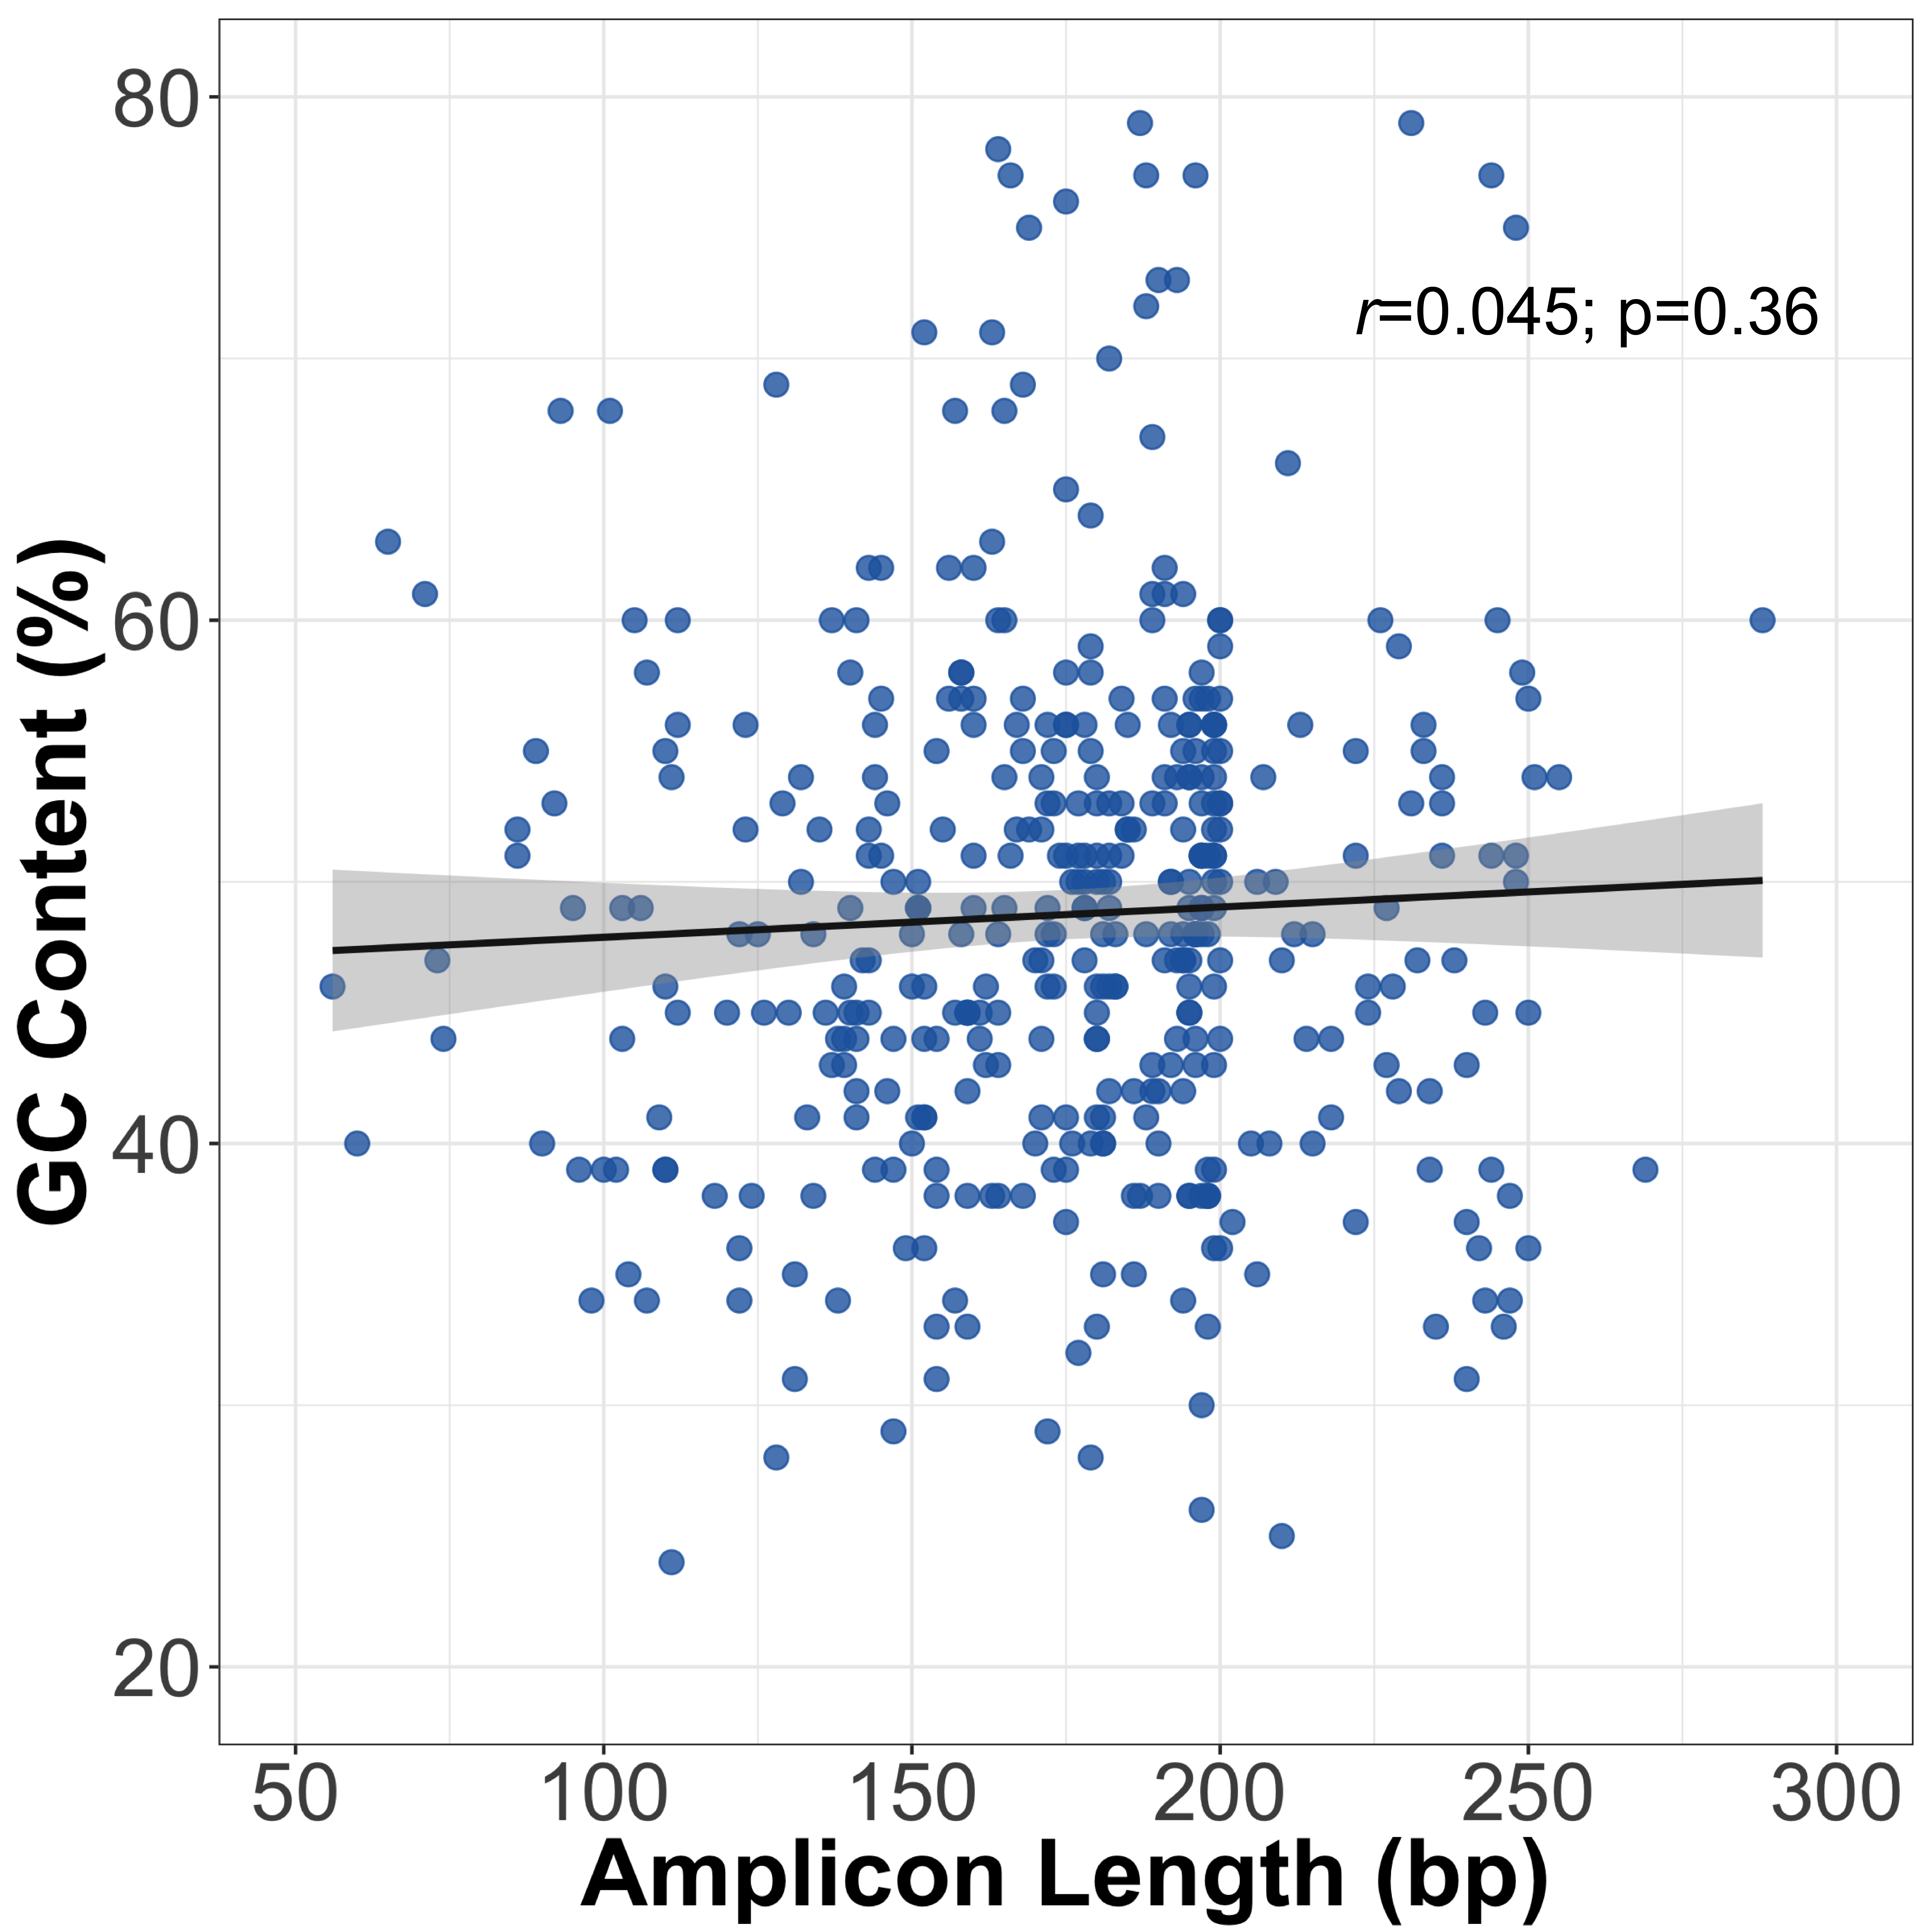
\includegraphics[scale=0.08]{amp_gc_length.png}
\end{figure}
\end{frame}

\begin{frame}
\frametitle{Research Question}
\begin{figure}[t]
    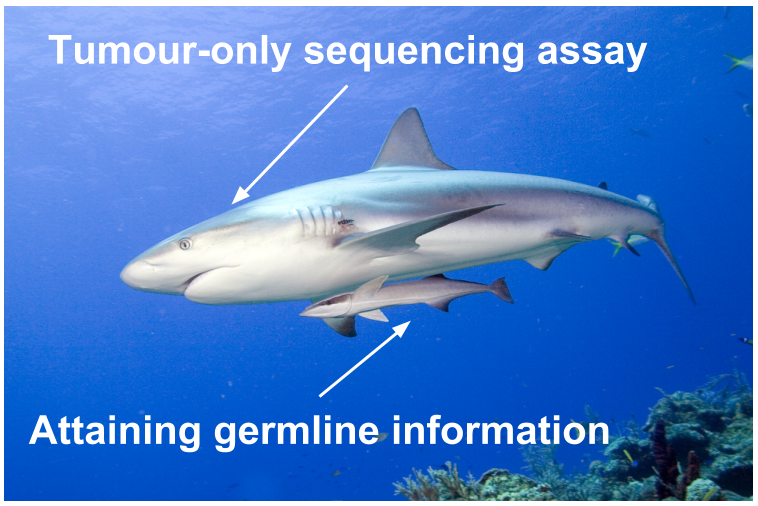
\includegraphics[scale=0.3]{clin_reality_shark.png}
\end{figure}
Can we leverage tumour genomic testing to perform screening for clinically relevant germline variants?
\end{frame}

\end{document}
